\chapter{绪论}
\section{背景与意义}

随着科技的进步,机器人技术近年来实现了飞速发展,其应用场景已从传统的工业制造领域,
迅速拓展至医疗、教育、军事、交通等更广阔的社会服务与民生领域。机器人技术已成为驱动
未来新兴产业发展和科技创新的关键基础,对促进国民经济增长和加强国防建设具有不可替代
的战略意义\cite{2013RobotProgress}。移动与操作是机器人需要实现的两个功能。
在各种机器人构型中,腿足式机器人因其仿生学设计,展现出卓越的环境适应性和通过能力,
能够灵活跨越障碍、稳定通过复杂路面,使其成为探险、搜救和野外作业等领域不可或缺的
理想平台\cite{孟健2015复杂地形环境四足机器人运动控制方法研究与实现}。但是在现实中,许多任务涉及操作任务,尽管腿足式机器人可以使用腿足完成推、拉等简单的
操作任务,这种方式通常会削弱机器人的移动能力,且难以在运动过程中进行精细化的操作。为四足机器人装配机械臂(Legged Manipulator System,简称LMS)成为了增强其作业能力的关键途径。机械臂的加入使得四足机器人从单纯的移动平台升级为了具备操作能力的多功能系统,能够执行远远操作仅仅使用腿足作为执行器的复杂精细的多样化任务。例如,在电力、油气等基础设施的巡检任务中,足式机械臂可以行走在复杂的管道或崎岖地面上,并利用机械臂搭载传感器或工具进行高精度仪表读数、阀门开关甚至简单故障的现场维修。在生活服务与辅助照护领域,足式机械臂能够稳定的跨过家庭环境中的地毯、门槛与楼梯场景,并利用机械臂完成捡垃圾、拿快递等任务\cite{bellicoso2019alma, wang2025quadwbggeneralizablequadrupedalwholebody}。在废墟荒地中,足式机械臂可以在碎石瓦砾上行走并利用机械臂携带检测仪器进行检测勘探等任务、甚至进行生命探测仪器的精确部署\cite{doi:10.1126/scirobotics.ade9548}。它们能够深入危险地带执行传统机器人无法完成的一体化复杂任务,极大地提高了检测效率和人员安全性。在图\ref{Fig.1.1}中,展示了当前足式机械臂在各种应用场景中执行上文中描述的清理勘探任务。
\begin{figure}[htbp]
      \centering
      \subfloat[]{
            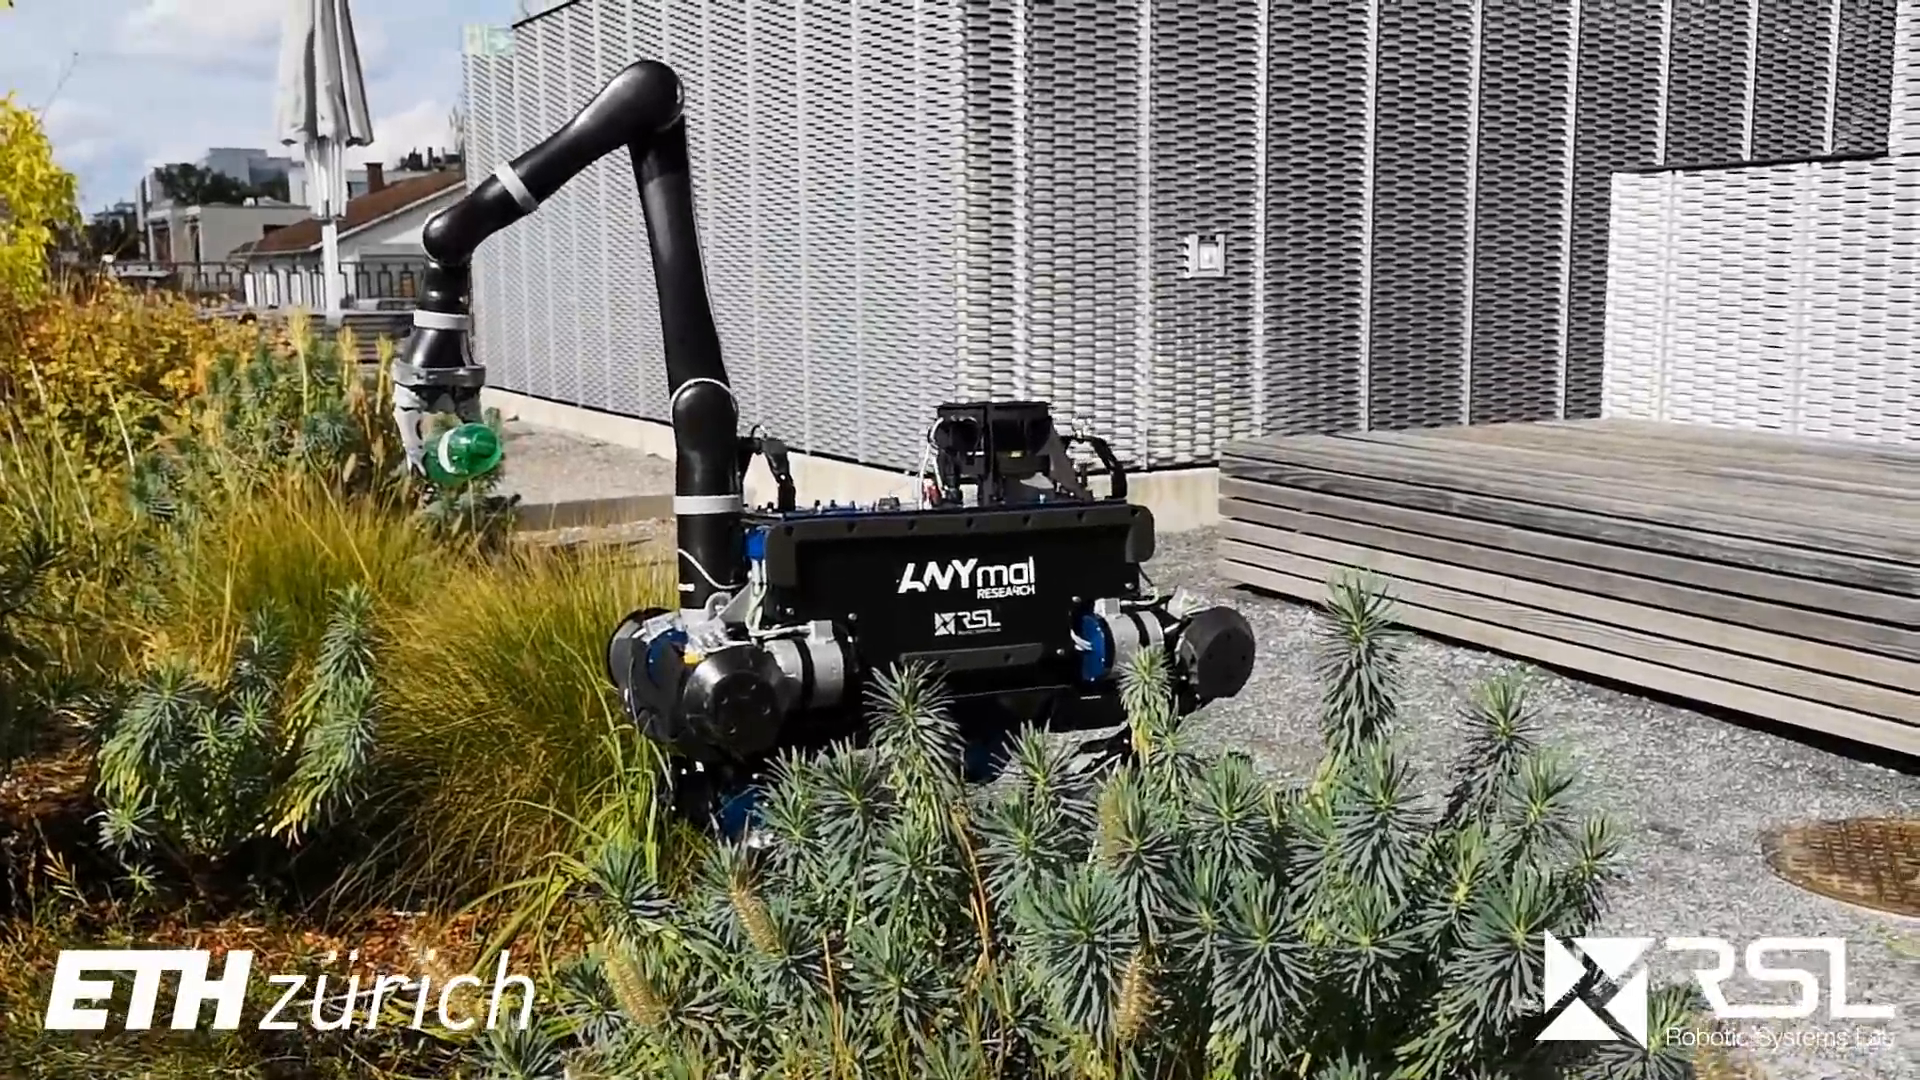
\includegraphics[width=0.32\textwidth]{content/alma.png}
      }
      \subfloat[]{
            \includegraphics[width=0.32\textwidth]{content/ecpa.png}
      }
      \subfloat[]{
            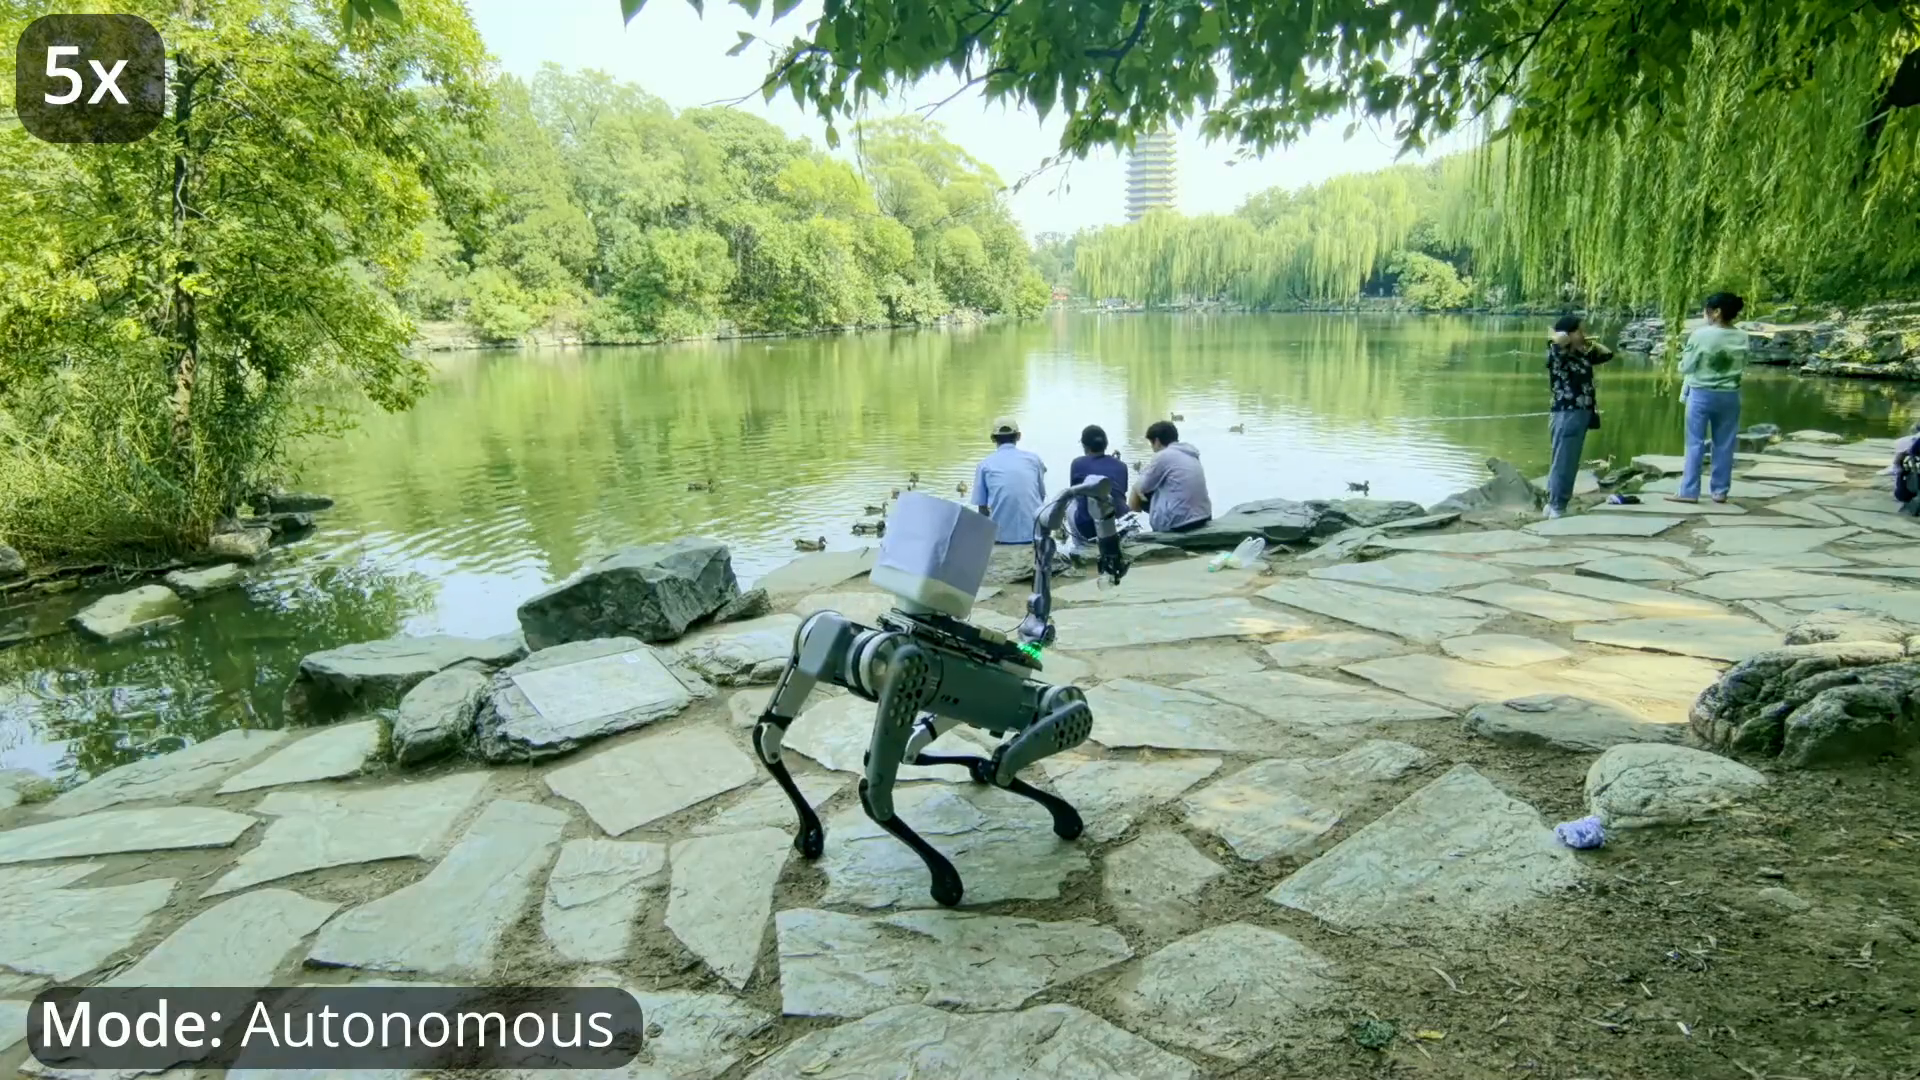
\includegraphics[width=0.32\textwidth]{content/qwbg.png}
      }
      \caption{足式机械臂能够在各种环境中执行清理垃圾,勘探与检测任务,具有广泛的应用场景}
      \label{Fig.1.1}
\end{figure}

然而,四足机械臂控制系统是一个高自由度、强耦合和高度非线性的动态系统,关于该构型的全身目标规划与全身协同控制仍然是当前研究中的关键难点。尤其在全身协同控制层面,机械臂的运动会对四足机器人稳定性会造成显著的扰动;同时,四足机器人还必须主动的进行步态调整与位姿配合,以扩展机械臂的操作空间,确保操作任务的成功执行。如果高效的解决这种多目标、强耦合的全身动态协调控制问题,是制约足式机械臂从理论走向实际应用的关键瓶颈。目前,模型预测控制(Model Predictive Control,简称MPC)是实现足式机械臂精确控制的主流方法。不过其控制方法存在显著的局限性:首先,它必须依赖于精确且复杂的全身动力学模型,这给建模过程带来了巨大的工程难度和不确定性;其次,MPC的计算复杂度高,难以在高度动态和实时环境(如复杂地形)中满足高频率的控制需求;此外,在机械臂末端执行器进行复杂操作时,还需要耗费巨大的工程努力来处理和避免奇异点等问题,以确保控制的稳定性和精度。相比之下,近年来,深度强化学习(Deep Reinforcement Learning, 简称DRL)在机器人控制领域,尤其是四足机器人运动控制方面,展现出强大的鲁棒性与环境适应性\cite{gu2017deep, kalashnikov2018scalable, chen2023visual, kim2024not, nahrendra2023dreamwaq}。DRL通过结合深度神经网络的强大拟合能力和强化学习的决策优化能力,使智能体通过与环境的大规模并行化仿真交互,自主学习并优化控制策略。这种基于数据驱动的控制范式,显著减少了对精确物理建模的依赖,提供了一种更加灵活、高效且鲁棒的全身控制解决方案。因此,深入研究基于深度强化学习的四足机械臂全身运动协同控制方法,对于推动该平台在复杂任务场景中的智能化和自动化应用具有重大的理论与实际意义。

综上所述,如何利用深度强化学习算法实现足式机械臂流畅且鲁棒的全身协同控制是本文的核心研究目标。
足式机械臂的全身协同控制问题可以被抽象为两个相互耦合的控制任务:
一是四足机器人的速度追踪运动控制;二是机械臂末端执行器的位姿追踪控制。
这两个任务是相互制约、紧密耦合的。具体而言,基座的动态运动会对机械臂的位姿跟踪
产生扰动,而机械臂的运动反过来也会对基座的稳定造成挑战。更重要的是,
为了让机械臂能够到达并稳定操作给定的目标位姿,基座必须流畅地做出主动配合行为
(如俯仰、侧倾),而这种配合行为的设计难度极高,且会对两个控制目标造成进一步的耦合影响。
针对上述挑战,本文提出一种基于深度强化学习的足式机械臂全身协同控制方法。
具体而言,我们利用机械臂的运动学模型,建立基座姿态与机械臂工作空间的可达性之间的映射关系,
并据此设计了物理可行性引导(Physical Feasibility Guidance, 简称PFG)奖励机制。
该机制通过实时判断当前躯干姿态是否能让机械臂在关节配置安全域内达到目标位姿,
从而有效约束并引导策略探索方向,最终实现了足式机械臂流畅、鲁棒的全身运动与操作协同。

\section{问题与挑战}
由于足式机械臂在物流、巡检、赈灾救援等领域展现出巨大的应用潜力,其复杂性对机器人的
控制与部署系统提出了更高的要求。基于前文对该系统特性和现有方法局限性的分析,
本文的主要研究内容聚焦于解决以下关键问题与挑战:

\textbf{足式机械臂全身协同控制:}由于MPC方法需要复杂的建模建模步骤、高昂
的计算开销,并且难以实现身体与手臂之间的自然流畅配合,这推动了研究向数据驱动的深度强化学习转型。
尽管DRL优势显著,但应用于足式机械臂的全身控制仍面临一些严峻的挑战:
\begin{itemize}
      \item 多目标耦合与次优收敛: 足式机械臂的全身控制涉及基座稳定运动和
            机械臂精确操作这两个强耦合的任务目标。DRL策略的优化依赖于奖励函数
            对两个目标的加权评估。然而,由于奖励函数的权衡设计难度极高,DRL算法难以在优化过程
            中有效平衡相互制约的任务。这导致训练出的策略容易过度倾向于某一特定任务,
            最终收敛到次优或局部最优解,严重影响了控制器最终性能。
      \item 探索效率与行为流畅性缺失: 现有的DRL协同控制方法在处理高维连续动作空间
            时,通常缺乏对系统物理可行性的先验指导,导致策略探索效率低下。已有的解耦训练
            或优势混合方法往往采用两阶段训练,训练耗时,且难以得到高度自然、流畅且具备
            高鲁棒性的全身协同行为,制约了策略的实用性。
      \item 高精度追踪的难以实现: 相比于MPC等基于模型的优化方法,DRL策略
            由于其固有的函数逼近误差和随机探索特性,在实现高精度、高收敛性的末端执行器
            位姿追踪任务时往往表现不佳。这种相对较低的追踪精确度,对于需要精细触碰、抓取
            或插入等操作任务的机械臂而言,是阻碍足式机械臂广泛应用的重要障碍。
\end{itemize}

\textbf{足式机械臂异构系统的Sim2Real部署鸿沟:}
足式机械臂系统本质上是一个异构系统:它将四足机器人与机械臂集成在一起。
这种异构性导致Sim2Real(仿真到现实)部署鸿沟被进一步放大。
\begin{itemize}
      \item 驱动器特性差异: 四足机器人通常采用大扭矩、低减速比的行星减速器电机,
            强调动态响应和功率密度;而机械臂则普遍采用高减速比、
            高精度的谐波减速器电机,强调刚度和高精度定位。
            这种显著的硬件差异导致其电机控制特性在仿真中难以被统一和精确建模。
      \item 高增益控制的仿真难度: 机械臂为了保证操作精度,需要使用较大
            的$K_p$和$K_d$增益进行控制。在仿真环境中,使用如此大的控制增益
            来精确模拟机械臂的电机控制特性极具挑战性,细微的建模误差在高增益下
            会被放大,导致在仿真中训练过程难以收敛,策略输出趋向于振荡,极大地制约
            了强化学习策略的实际部署。
\end{itemize}

\textbf{全身控制系统的故障容错与鲁棒性架构设计:}
在现实世界的任务执行中,故障障容错能力和系统鲁棒性是足式机械臂从实验室走向实
际应用的关键指标。足式机械臂的复杂性要求其能够在执行操作时,有效地应对子系统(机械臂)
的突发性故障,避免控制系统崩溃。
\begin{itemize}
      \item 功能解耦与故障隔离挑战: 尽管足式机械臂的控制目标是高度耦合的,
            但其控制主体(基座与机械臂)在控制逻辑上应实现故障隔离。
            具体而言,当机械臂因电机过热或传感器故障等问题
            导致控制失效时,控制系统不应因该子系统的故障而崩溃,
            而是需要迅速克服机械臂失控带来的扰动,保持基座的稳定运动控制,
            从而将故障机械臂安全地转移到收纳或维修位姿。
      \item 鲁棒性架构与先验知识的局限: 基于模型的传统方法(如MPC)
            通常将足式机械臂视为一个单一体、完全耦合的系统进行优化,其控制律依赖
            于模型的假设,本质上缺乏对子系统故障的内在感知和应对机制。
            虽然深度强化学习(DRL)作为一种数据驱动的方法,
            有可能通过在仿真中注入故障数据来学习相应的故障容错策略和解耦状态,
            但如何高效、系统性地构建并验证这种具备故障容错能力的DRL架构,
            仍是一个问题。
\end{itemize}

\textbf{非结构化环境中的动态全身控制与感知融合:}
足式机械臂的最终应用场景是户外、灾区或家庭等典型的非结构化环境。在这些场景中,足式机械臂不仅要克服
复杂、动态变化的崎岖地形如碎石、泥泞、楼梯,还必须使用机械臂在移动过程中进行相应操作任务。
\begin{itemize}
      \item 高动态全身协同控制的实时性与鲁棒性:在复杂地形上保持稳定移动本身就是一项
            高动态控制难题。当系统同时执行全身协同操作时,需要在极高频率的运动控制环中实时
            融合环境感知、本体状态和操作目标信息。实现基座动态稳定与机械臂操作一体化的控制系统,
            对算法的提出了极高的要求。
      \item 感知不确定性与地形适应性挑战:非结构化环境中的传感器数据不可避免地存在
            噪声、漂移和遮挡(即感知不确定性)。足式机械臂需要智能地在依赖感知的模式
            与不依赖感知的盲走模式之间进行鲁棒切换,以适应环境变化。此外,为了在复杂
            地形上扩展机械臂的工作空间或保持身体稳定,系统必须具备强大的全身协同能力,
            以在满足操作约束的同时,确保足端与地面的物理可行性接触,
            并利用机械臂完成相应操作任务。
\end{itemize}

\section{本文研究内容与贡献}

基于上述全身控制器面临的关键挑战,本文围绕基于强化学习的足式机械臂全身协同运动
控制方法、异构系统sim2real方法、物理可行域引导的奖励设计方法、与基于空间注意
力的感知融合方法展开研究。

在足式机械臂的全身控制架构方法,我们采用了PPO强化学习算法,使用了非对称性Actor-Critic架构。
在训练过程中,Actor与Critic网络接受的输入完全不一样。Critic没有任何的部署的需求,因此接受
理想无噪声的机器人状态数据,这些状态数据可以直接从仿真中获取。这种方法使得Critic估计的Value
值更加准确,从而高效的指导策略收敛。而Actor网络(即策略网络)的输入则严格受限于在真实机器人上
可获取的信息,这确保了策略的直接可部署性。实验证明采用非对称性的网络结构设计能够加速收敛,提升
训练效率与最终策略的效果。

在此基础上,为了弥补足式机械臂控制系统在仿真域现实之间的巨大鸿沟,我们采用了分离式框架设计,
结合域随机化与课程设计方法,通过对各个传感器收集的数据加入噪声和延迟,来模拟真实机器人上的
传感器数据。例如:对于机器人控制器,我们采用了双延迟缓冲器的设计来模拟控制延迟。对于机器人关节
状态数据,我们通过单延迟缓冲器与引入高斯噪声来模拟真实机器人上获得的关节状态数据。
对于地形感知数据,我们模仿elevation mapping地图更新方法,
通过内部维护部分一个局部地图,来模拟在真实机器人上获得的地形感知数据。
除此之外,机械臂与四足机器人采用的电机不同,相比四足机器人的电机,机械臂采用了谐波减速器,需要极大的
$K_p$与$K_d$增益来实现高精度的控制。在仿真训练中,策略网络的微小输出被较大的$K_p$与$K_d$
放大,导致机械臂运动振荡,这使得训练的策略难以部署在真实的机器人上。为了解决这个问题,
我们引入了虚拟力奖励引导机制,力矩奖励并非由机械臂真实的控制力矩生成,而是由一个理想pd控制器生成,
尽管该力矩并不是真正的作用在机械臂上。但是在优化过程中,这个奖励可以让策略网络学习
到PD控制器位置与力的关系,进而改变输出幅值,减轻振荡效应。

操作与移动的全身协同控制问题是足式机械臂控制中的关键难点。
在学习过程中,策略往往难以学习身体与手臂的配合行为,原因是,身体的配合会对四足机器人
的速度追踪任务产生负面影响,为了获得更好的速度追踪性能,策略往往会忽略身体的配合行为,
此时策略逐渐收敛至局部最优。
针对现有DRL方法在平衡“稳定移动”和“精确操作”两大耦合目标时容易收敛至局部最优的局限。
本文提出了基于物理可行域引导的奖励设计方法。该方法借鉴生物体在移动中进行操作的
协同原理,将显式的机器人运动学模型作为先验知识引入奖励函数。
在训练过程中,当身体状态使得操作任务可达时,该身体状态被是视为一个可行身体状态。
策略不仅仅追求任务奖励的最大化,还需要探索并保留在给定操作任务下的可行
身体状态。该方法能有效的引导了策略探索方向,使得策略收敛避开局部最优解,最终实现了足式
机械臂流畅、鲁棒的全身运动与操作协同。

此外,足式机械臂在非结构化场景中面临的传感器不确定性和故障容错挑战,我们设计了一种基于
空间注意力机制的网络模型,以实现机器人内部状态与环境感知的鲁棒融合。该模型利用空间注意
力机制动态调整网络对环境感知信息的权重,并结合门控神经网络结构,实现了对感知信息的鲁棒
处理。当外部感知数据因噪声或故障而不可用时,网络能够智能地退化为基于内部状态的无感知模式。
这种动态的鲁棒切换能力,有效增强了全身控制器的环境适应性与故障容错能力,确保了足式机械臂
在复杂地形上执行操作任务的可靠性。

\section{本文结构}
本文共有六章,结构安排如下:

第一章主要介绍了足式机械臂系统的发展背景与研究意义,明确指出了当前足式机械臂全身协同控制中的常用方法与该领域面临的技术挑战,并概述了本文的研究动机、主要内容与核心贡献。

第二章详细介绍了与足式机械臂全身控制相关的模型预测控制与强化学习理论知识,详细介绍了基于MPC的足式机械臂的全身控制方法与基于强化学习的全身控制方法,分析了当前足式机械臂全身控制领域的研究现状,评述了各自的优势与不足,从而为后续研究内容奠定基础。

第三章介绍了足式机械臂具体的控制任务、仿真环境与网络结构设计。

\chapter{足式机械臂全身控制方法概述}

\section{引言}

四足机械臂全身控制任务被分解为两个控制任务,一个是四足机器人的运动控制,即希望
四足机器人能够在给定速度指令下稳定行走。第二是机械臂的位姿控制,给定机械臂末端
执行器的目标位姿,希望机械臂尽快的到达该目标位姿并保持稳定。在实际任务中,两者
高度耦合。比如在四足机器人站立姿态下,机械臂的工作空间受到限制,为了扩展
机械臂的工作空间,四足机器人的身体姿态也需要满足相应的要求。在学界,足式机械臂的
全身控制主要分为基于MPC的控制方法与基于强化学习的控制方法两大类。MPC 依赖于
精确的动力学模型和高效的实时优化求解器,能够显式处理复杂的动力学约束
和接触力约束,提供运动轨迹的可行性和理论保证。由于足式机械臂的接触状态(脚和地面的接触
状态,机械臂末端执行器与操作物体的接触状态)是不断切换的,因此MPC将多点接触系统建模
为切换系统,并依赖优化器进行实时的求解。对模型与优化的强依赖性导致MPC方法控制效果不过
鲁棒,尤其优化器十分耗时,难以满足实时性要求。
深度强化学习(DRL)为足式机械臂全身控制提供了一条无需精确物理建模的路径。
通过端到端学习,DRL 能够训练出高度鲁棒且生物学上协同的统一策略,有效应对
高维度动作空间和复杂动力学耦合。因此,本文基于强化学习,通过设计合理的奖励函数与网络结构,
实现流畅鲁棒的强化学习全身控制器。本章详细介绍了现有足式机械臂的主要平台,并分析了现有
平台控制方法的优点与缺点。
% 然后对强化学习相关内容进行介绍,为本文后续内容做好基础讲解。

\section{足式机械臂硬件平台}

足式机械臂系统是移动操作机器人领域的重要分支,其本质是在四足移动机器人的躯干上
集成一个或多个多自由度机械臂,从而构成具备“移动”与“操作”双重能力的复合系统。
% 与传统的轮式或履带式移动操作平台相比,四足底盘摆脱了对连续平坦地面的依赖,
% 能够适应台阶、碎石等非结构化地形,显著拓展了机器人的作业空间。
% 而相较于双足人形机器人,四足底盘拥有更大的支撑多边形和更低的重心,在执行大负载
% 操作或高动态全身运动时,具备天然的静态与动态稳定性优势。
近年来,随着高功率密度电机、高能量密度电池以及轻量化材料技术的突破,足式机器人的
负载能力得到了显著提升,使其搭载机械臂成为可能。针对不同的应用需求与控制策略,
国内外多家顶级实验室与商业公司研发了多种形态各异的四足机械臂平台。
本节将重点回顾几类具有代表性的实验平台,并分析其硬件特性及优劣势。

\subsection{国外足式机械臂硬件平台}
2015年2月,波士顿动力发布了第一代名为 Spot(Spot Classic)的四足机器人,
该平台首次展示了四足机器人在室内狭窄空间与室外复杂地形下的卓越运动能力,
标志着高爆发电驱动技术在足式机器人领域的成熟应用\cite{ackerman2015spot}。
为了进一步适应非结构化的人居环境并拓展移动操作能力,波士顿动力于2016年6月
推出了SpotMini\cite{bostondynamics2016mini}。作为当前商业化 Spot 的直接原型,SpotMini 是首
个在四足底盘上深度集成全电动机械臂的实验平台,确立了“移动操作”的技术范式。
在控制架构方面,Spot 系列展现了卓越的全身协调控制能力。尽管具体实现细节
未完全公开,但业界普遍认为其沿用了波士顿动力在 Atlas 人形机器人上验证
成熟的分层式控制架构\cite{kuindersma2016optimization}:底层基于高频阻抗控制
律实现关节级的柔顺性与力矩跟踪;上层核心则广泛应用模型预测控制(MPC)来处理
非线性倒立摆模型的稳定性问题\cite{kuindersma2016optimization,}。特别是在涉及机械臂大动量操作
(如抛掷重物或开启重型门)的任务中,系统能够构建全身动力学方程,将机械臂运动
产生的反作用力与倾覆力矩作为前馈项引入底盘控制器,通过主动调整步态、支撑多边形
及关节力矩来维持系统平衡。

2018年,波士顿动力展示了 SpotMini 利用机械臂自主开启重型弹簧门的实验记录
,SpotMini 通过躯干的主动俯仰配合机械臂的末端轨迹,成功克服了弹簧阻力\cite{bostondynamics2018opendoor}。
在执行过程中,面对外界施加的强烈干扰,控制器能够实时调整全身姿态,
展现了极强的鲁棒性。然而,由于 Spot 系统的底层关节力矩控制器处于闭源状态,
且硬件成本高昂,其核心控制算法对学术界呈现“黑盒”特性\cite{gupta2021embodied}。
这在一定程度上限制了科研人员在该平台上直接验证底层全身动力学或端到端
强化学习力矩控制策略的可能性。

苏黎世联邦理工学院(ETH Zurich)研发的 ANYmal 系列及其衍生的 ALMA
(Articulated Locomotion and Manipulation)系统,代表了当前足式机械臂全身控制
研究在学术界的最高水准。与商业化平台不同,该系统自研发之初便强调驱动器的控制架构的开放性,
旨在解决高动态移动操作中的强耦合动力学问题\cite{hutter2016anymal}。

在硬件演进方面,ALMA 系统经历了从集成商用组件到全栈自研的过程。早期的 ALMA 系统
(约 2018 年)基于 ANYmal B 四足底盘,集成了 Kinova Jaco 轻量级机械臂。
尽管该配置验证了基本的全身协调算法,但由于商用机械臂的低带宽位置控制模式,
难以实现高频的力交互操作\cite{bellicoso2019alma}。为了突破这一瓶颈,ETH 团队
随后研发了专用的 DynaArm 机械臂\cite{sleiman2021unified,ma2022combining,sleiman2023versatile},其采用了与 ANYmal 腿部
关节一致的高扭矩密度驱动技术。这一硬件升级使得系统能够感知微小的外界接触力,
为后续的高动态任务提供了物理基础。

在控制算法层面,该平台见证了从基于模型的预测控制(MPC)向基于强化学习(RL)的范式转移。
早期的研究主要采用非线性模型预测控制(NMPC)架构,通过构建全身动力学约束方程,
实时优化底盘步态与机械臂轨迹,成功实现了开启重型弹簧门、协同搬运等任务\cite{bellicoso2019alma},
之后,该控制框架引入规划模块,实现了身体与机械臂、腿足与机械臂的配合效果,在结构化场景
中可以完成多种操作任务\cite{sleiman2021unified,sleiman2023versatile}。
然而,面对非结构化环境中的接触不确定性,基于模型的规划往往面临建模误差的挑战。
近年来,随着深度强化学习的发展,该团队在 ANYmal 平台上展示了基于学习的全身协同策略。
最新的研究成果显示,通过在物理仿真中进行大规模端到端(End-to-End)训练,
机器人能够掌握极具挑战性的高动态全身运动操作技能,如模拟照顾残疾人的精细抓取以及
涉及快速挥臂的类体育运动任务\cite{scheidemann2024cybathlonleggedmobile,doi:10.1126/scirobotics.adu3922}。
这些算法不仅利用了身体的配合姿态来扩展机械臂作业空间,还通过本体感知实现了对外界
扰动的自适应鲁棒控制。尽管该平台在性能上具备显著优势,但其高昂的硬件成本与复杂
的维护需求,限制了其在工业场景中的大规模普及,目前仍主要作为验证前沿控制理论的
科研载体。

\subsection{国内机械臂硬件平台}

自2017年以来,随着国内机器人产业链的成熟与高功率密度电机技术的突破,中国在足式机器人
领域迅速发展,涌现出以宇树科技(Unitree Robotics)和云深处科技(Deep Robotics)
为代表的领军企业。这些国产平台凭借准直驱(Quasi-Direct Drive, QDD)技术的广泛应用、
高度开放的底层控制接口以及模块化的硬件架构,迅速被全球科研机构采用,极大地推动了基于
强化学习的全身控制算法从仿真走向真机(Sim-to-Real)的验证进程。

在众多平台中,宇树科技研发的系列四足机器人(如 Aliengo, B1, Go2)配合其自研的Z1机
械臂,构成了当前学术界最为通用的实验载体。特别是Z1机械臂,专为移动机器人设计,具有
极高的力矩自重比和与底盘一致的控制协议。研究人员利用该平台,能够将四足底盘与机械臂
视为统一的动力学系统,在仿真环境(如 Isaac Lab)中进行大规模并行训练,进而将端到
端的神经网络策略直接部署于物理样机\cite{fu2022coupling, ji2022concurrent}。
这种全栈式的硬件生态解决了以往异构系统中通信延迟高、控制带宽不匹配的难题。

另一方面,云深处科技推出的“绝影”(Jueying)系列机器人(如 X20, X30)则深耕工业
巡检与特种作业场景。该类平台强调复杂地形下的运动稳定性与高负载能力,常被用于验证基于
模型预测控制(MPC)的重载移动操作任务。尽管其部分底层接口主要面向行业应用优化,
但其稳定的状态估计与运动原语为上层长周期规划算法提供了可靠的验证环境\cite{wang2021model}。

此外,随着轮足复合技术的兴起,国内亦出现了如逐际动力(LimX Dynamics)W1等新型移动
操作平台,进一步丰富了足式机械臂的研究形态。
综上所述,国产高性能平台的普及降低了全身控制研究的硬件门槛,
但轻量化平台中显著的机臂惯性耦合效应,也对控制算法的抗扰动能力提出了更高的要求。


\section{足式机械臂控制方法概述}

\subsection{模型预测控制}

\subsubsection{分层控制框架}
在动力学建模层面,为了平衡计算效率与预测精度,MPC 规划层通常采用扩展的单刚体动力学模型。与传统仅将底盘视为刚体的方法不同,该模型将底盘与机械臂视为一个具有时变惯量特性的复合刚体系统。

设系统的状态向量为 $\mathbf{x} \in \mathbb{R}^n$,控制输入向量为 $\mathbf{u} \in \mathbb{R}^m$。状态向量 $\mathbf{x}$ 包含全身复合质心位置 $\mathbf{p}_{\text{com}}$、质心速度 $\mathbf{v}_{\text{com}}$、基座姿态欧拉角 $\boldsymbol{\Theta}_b$、基座角速度 $\boldsymbol{\omega}_b$ 以及机械臂的关节角度 $\mathbf{q}_{\text{arm}}$ 与关节速度 $\dot{\mathbf{q}}_{\text{arm}}$。系统的动力学演化遵循牛顿-欧拉方程,其具体形式如下:
\begin{subequations}
      \begin{align}
            \dot{\mathbf{p}}_{\text{com}}                                                                      & = \mathbf{v}_{\text{com}}                                                                                                               \\
            m_{\text{sys}} \dot{\mathbf{v}}_{\text{com}}                                                       & = \sum_{i=1}^{n_c} \mathbf{f}_i + m_{\text{sys}} \mathbf{g} \label{eq:linear_dyn}                                                       \\
            \frac{d}{dt} \left( \mathbf{I}_{\text{sys}}(\mathbf{q}_{\text{arm}}) \boldsymbol{\omega}_b \right) & = \sum_{i=1}^{n_c} (\mathbf{r}_i - \mathbf{p}_{\text{com}}) \times \mathbf{f}_i + \boldsymbol{\tau}_{\text{ext}} \label{eq:angular_dyn}
      \end{align}
\end{subequations}
其中,式(\ref{eq:linear_dyn}) 描述了线性动量变化率,式(\ref{eq:angular_dyn}) 描述了角动量变化率。

为了构建适用于模型预测控制的标准状态空间模型,我们需要将上述物理方程重写为一阶微分形式。通过结合机械臂的运动学关系 $\dot{\mathbf{q}}_{\text{arm}} = \mathbf{v}_{\text{arm}}$,并将式(\ref{eq:linear_dyn})与式(\ref{eq:angular_dyn})整理为关于状态导数 $\dot{\mathbf{v}}_{\text{com}}$ 与 $\dot{\boldsymbol{\omega}}_b$ 的显式表达式,可得到系统的非线性状态空间方程:
\begin{equation}
      \dot{\mathbf{x}}(t) =
      \begin{bmatrix}
            \dot{\mathbf{p}}_{\text{com}} & \dot{\mathbf{v}}_{\text{com}} & \dot{\boldsymbol{\Theta}}_b & \dot{\boldsymbol{\omega}}_b & \dot{\mathbf{q}}_{\text{arm}} & \ddot{\mathbf{q}}_{\text{arm}}
      \end{bmatrix}^T
      = f(\mathbf{x}(t), \mathbf{u}(t))
      \label{eq:state_space_func}
\end{equation}
该函数 $f(\cdot)$ 完整映射了系统状态随控制输入的演化规律。需要特别指出的是,方程中的 $\mathbf{I}_{\text{sys}}(\mathbf{q}_{\text{arm}}) \in \mathbb{R}^{3 \times 3}$ 表示系统的复合刚体惯性张量。与传统四足机器人恒定的躯干惯量不同,足式机械臂的惯性分布会随着机械臂关节角度 $\mathbf{q}_{\text{arm}}$ 的变化而显著改变。因此,在推导 $\dot{\boldsymbol{\omega}}_b$ 时(即构建函数 $f$ 的角速度分量时),必须将角动量的变化率展开为包含陀螺力矩项的形式:
\begin{equation}
      \mathbf{I}_{\text{sys}}(\mathbf{q}_{\text{arm}}) \dot{\boldsymbol{\omega}}_b + \underbrace{\left( \boldsymbol{\omega}_b \times \mathbf{I}_{\text{sys}}(\mathbf{q}_{\text{arm}}) \boldsymbol{\omega}_b + \dot{\mathbf{I}}_{\text{sys}}(\mathbf{q}_{\text{arm}}, \dot{\mathbf{q}}_{\text{arm}}) \boldsymbol{\omega}_b \right)}_{\text{非线性耦合项}} = \boldsymbol{\tau}_{\text{total}}
\end{equation}
上式清晰地表明,机械臂的快速运动(体现为 $\dot{\mathbf{q}}_{\text{arm}}$ 导致的 $\dot{\mathbf{I}}_{\text{sys}}$ 项)会直接在基座上产生附加的惯性力矩耦合。如果忽略这一时变特性,将 $\mathbf{I}_{\text{sys}}$ 视为常数,则会在 MPC 预测视界内引入显著的模型误差。

基于上述建立的状态空间模型 $f(\mathbf{x}, \mathbf{u})$,模型预测控制的核心在于在每一个控制周期内,求解一个有限时间视界 $T$ 内的开环最优控制问题。该优化问题旨在寻找最优控制序列 $\mathbf{u}^*(\cdot)$,使得系统的状态轨迹在满足物理约束的前提下尽可能跟踪参考轨迹。其数学表达如下所示:
\begin{subequations}
      \begin{align}
            \min_{\mathbf{u}(\cdot)} \quad & \int_{0}^{T} \left( \|\mathbf{x}(t) - \mathbf{x}_{\text{ref}}(t)\|_{\mathbf{Q}}^2 + \|\mathbf{u}(t)\|_{\mathbf{R}}^2 \right) dt + \|\mathbf{x}(T) - \mathbf{x}_{\text{ref}}(T)\|_{\mathbf{P}}^2 \\
            \text{s.t.} \quad              & \dot{\mathbf{x}}(t) = f(\mathbf{x}(t), \mathbf{u}(t)) \label{eq:dynamics_constraint}                                                                                                            \\
                                           & \mathbf{f}_i(t) \in \mathbb{C}(\mu, \mathbf{n}) \quad \forall i \in \{1, \dots, n_c\} \label{eq:friction}                                                                                       \\
                                           & \mathbf{p}_{\text{foot}, i}(t) \in \mathbb{S}_{\text{terrain}} \label{eq:terrain}                                                                                                               \\
                                           & \mathbf{x}_{\text{min}} \leq \mathbf{x}(t) \leq \mathbf{x}_{\text{max}}, \quad \mathbf{u}_{\text{min}} \leq \mathbf{u}(t) \leq \mathbf{u}_{\text{max}} \label{eq:limits}
      \end{align}
\end{subequations}
上述公式中,目标函数包含过程代价与终端代价,矩阵 $\mathbf{Q}, \mathbf{R}, \mathbf{P}$ 分别为状态误差、控制输入及终端误差的权重矩阵。约束条件(\ref{eq:dynamics_constraint})即为前文推导的包含惯性耦合效应的系统动力学约束;式(\ref{eq:friction})为接触力摩擦锥约束,确保足端不发生打滑;式(\ref{eq:terrain})为地形几何约束,限制落足点在可行区域内;式(\ref{eq:limits})为关节位置、速度及力矩的物理限位约束。

由于 MPC 规划层的更新频率通常较低,且基于简化模型,为了实现高频且精准的运动执行,控制系统下层通常配备一个基于全阶动力学的全身控制器(WBC)。WBC 接收 MPC 输出的期望反作用力 $\mathbf{f}_{\text{mpc}}$ 与运动轨迹 $\mathbf{x}_{\text{mpc}}$,通过求解二次规划(Quadratic Programming, QP)问题,将任务空间的加速度指令映射为各关节的力矩指令 $\boldsymbol{\tau}$。该层级能够利用全身冗余自由度处理任务优先级,例如在保证质心平衡的首要任务下,尽可能减小机械臂末端的操作误差。这种分层递阶的控制架构有效地解决了足式机械臂长时间跨度规划与瞬时高频响应之间的矛盾,构成了基于模型控制方法的核心逻辑\cite{bledt2018policy, bellicoso2017dynamic}。

\subsubsection{基于MPC分层控制框架的足式机械臂全身控制}
基于上述分层控制理论,早期的足式机械臂研究往往采用解耦的控制策略,即将机械臂视为对四足底盘的外部扰动,或仅在运动学层面进行协调。然而,当机械臂执行快速挥动或重载操作时,忽略两者之间的动力学耦合会导致底盘稳定性显著下降。针对这一问题,苏黎世联邦理工学院的研究团队在ALMA\cite{bellicoso2019alma}平台上提出了一系列改进方案,实现了从解耦控制向统一全身控制的跨越。

2021年,Sleiman 等人提出了一种统一全身 MPC 框架\cite{sleiman2021unified},其核心创新在于扩展了系统的状态空间与动力学模型。与传统方法仅将身体视为单刚体不同,该框架将机械臂的关节位置 $\mathbf{q}_{arm}$ 与速度 $\dot{\mathbf{q}}_{arm}$ 显式纳入 MPC 的预测状态向量 $\mathbf{x}$ 中。此时,系统的全身惯性张量 $\mathbf{I}(\mathbf{q}_{arm})$ 不再被视为常数,而是被建模为随机械臂构型变化的函数。在优化目标函数中,引入了针对机械臂末端位置 $\mathbf{p}_{ee}$ 的跟踪项:
\begin{equation}
      J_{track} = \int_{0}^{T} \left( \|\mathbf{p}_{com} - \mathbf{p}_{com}^{ref}\|_{\mathbf{Q}_{base}}^2 + \|\mathbf{p}_{ee}(\mathbf{q}_{arm}) - \mathbf{p}_{ee}^{ref}\|_{\mathbf{Q}_{arm}}^2 \right) dt
\end{equation}
通过联合优化四足机器人与机械臂的运动,该控制器能够产生涌现式的协同行为。例如,当机械臂试图抓取超出当前作业空间的物体时,MPC 会自动规划出身体前倾或调整步态的策略,利用全身冗余度来扩展操作范围,而无需人为指定底盘的配合动作。

在此基础上,Mittal 等人进一步提出了多接触规划与控制框架\cite{sleiman2023versatile},旨在解决涉及复杂环境交互的“移动操作”问题。该方法将足式机械臂系统建模为混合动力学系统,不仅考虑足端的地面反作用力,还将机械臂末端与环境的接触力 $\mathbf{f}_{ee}$ 纳入质心动力学方程:
\begin{equation}
      \dot{\mathbf{h}}_{com} = \sum_{i=1}^{n_{foot}} \mathbf{f}_{foot, i} + \mathbf{f}_{ee} + m\mathbf{g}
\end{equation}
该框架引入了开关系统理论来处理接触模式的离散切换,允许求解器在“仅足端支撑”与“足-手同时支撑”等模式间进行决策。在 ANYmal 机器人的硬件实验中,该方法成功实现了利用全身惯量开启重型弹簧门、在非平整地形上推拉重物以及利用墙壁支撑保持平衡等高动态任务,验证了基于模型的统一规划方法在处理复杂力交互方面的有效性。

尽管基于 MPC 的全身控制方法在理论完备性与可解释性上表现优异,但在实际应用中仍面临显著的局限性,这也推动了学术界向强化学习方向的探索:
\begin{itemize}
      \item \textbf{对模型精度的强依赖}:MPC 的性能高度依赖于动力学模型 $f(\mathbf{x}, \mathbf{u})$ 的准确性。在涉及抓取未知质量物体或在松软地面行走的场景中,惯性参数与摩擦系数的估计误差会导致预测轨迹与实际严重偏离,甚至引发系统发散。
      \item \textbf{非线性优化的实时性瓶颈}:为了处理全动力学约束,非线性 MPC 通常需要极其昂贵的计算资源。为了保证控制频率,现有的实现往往不得不缩短预测视界或简化模型,限制了机器人执行大跨度、高爆发动作的能力。
      \item \textbf{接触序列的预定义限制}:目前的 MPC 框架大多需要预先人为指定接触顺序。在极端复杂的非结构化环境中,依靠优化算法自主发现全新的接触策略(如意外摔倒时的支撑保护)仍然极其困难。
\end{itemize}
正是由于上述局限性,无需显式建模且具备在大规模数据中自主涌现复杂策略能力的强化学习方法,逐渐成为解决足式机械臂全身控制问题的新研究热点。

\subsection{强化学习}

强化学习作为机器学习的重要分支之一,其理论框架受到动物行为心理学与现代最优控制理论的影响。从爱德华·桑代克提出的“效果律”——即带来满意结果行为应被奖励,到理查德·贝尔曼在控制理论中奠定的动态规划基础,强化学习逐渐发展为一种通用的决策优化方法。它主要研究智能体如何在未知或部分未知的环境中,通过序列决策与试错机制,学习出能够最大化长期累积奖励的最优策略。

\subsubsection{强化学习问题建模与贝尔曼方程}

在足式机械臂的全身控制任务中,机器人的决策过程可以被建模为一个无限视界的马尔可夫决策过程(Markov Decision Process, MDP)。MDP 提供了一个标准化的框架来描述处于随机动态环境中的交互过程。

一个标准的马尔可夫决策过程由五元组 $\mathbb{M} = \langle \mathbb{S}, \mathbb{A}, \mathbb{P}, \mathbb{R}, \gamma \rangle$ 定义,其中各个元素物理意义如下:

\textbf{1. 状态空间 $\mathbb{S}$}
状态空间 $\mathbb{S}$ 定义了环境所有可能状态的集合。针对足式机械臂这一高维非线性系统,$\mathbb{S} \subseteq \mathbb{R}^n$ 是一个连续的欧几里得空间。时刻 $t$ 的状态向量 $s_t \in \mathbb{S}$ 通常包含机器人的本体感知信息,具体包括:基座的线性速度与角速度、重力向量在基座坐标系下的投影、各关节的角度位置以及角速度等。状态 $s_t$ 必须具备马尔可夫性,即包含预测未来所需的所有历史信息。

\textbf{2. 动作空间 $\mathbb{A}$}
动作空间 $\mathbb{A}$ 定义了智能体可执行的所有行为的集合。在连续控制任务中,$\mathbb{A} \subseteq \mathbb{R}^m$。时刻 $t$ 的动作向量 $a_t \in \mathbb{A}$ 直接对应于机器人的控制指令,常见的形式包括关节的目标位置、速度或力矩。

\textbf{3. 状态转移概率 $\mathbb{P}$}
状态转移概率 $\mathbb{P}: \mathbb{S} \times \mathbb{A} \times \mathbb{S} \rightarrow [0, \infty)$ 描述了环境的随机动力学模型。它表示在当前时刻 $t$ 处于状态 $s_t$ 并执行动作 $a_t$ 后,下一时刻 $t+1$ 系统状态服从的概率密度函数:
\begin{equation}
      s_{t+1} \sim \mathbb{P}(\cdot | s_t, a_t)
\end{equation}
对于足式机器人,该转移过程隐含了刚体动力学方程、地面接触模型以及摩擦约束,通常是高度非线性且难以解析建模的。

\textbf{4. 奖励函数 $\mathbb{R}$}
奖励函数 $\mathbb{R}: \mathbb{S} \times \mathbb{A} \rightarrow \mathbb{R}$ 是强化学习的核心引导信号。在每一时间步 $t$,智能体根据当前状态和动作获得一个标量即时奖励 $r_t = \mathbb{R}(s_t, a_t)$。该函数将复杂的控制目标(如保持平衡、跟踪速度、最小化能耗)量化为数值信号,直接决定了策略的学习方向。通常在强化学习中使用回报 $G_t$ 来评估策略在长期运行中的表现。$G_t$ 被定义为从时刻 $t$ 开始,未来所有时间步的折扣奖励之和:
\begin{equation}
      G_t = r_t + \gamma r_{t+1} + \gamma^2 r_{t+2} + \dots = \sum_{k=0}^{\infty} \gamma^k r_{t+k}
\end{equation}

\textbf{5. 折扣因子 $\gamma$}
折扣因子 $\gamma \in [0, 1)$ 用于权衡即时奖励与长期奖励的相对重要性。在数学上,$\gamma < 1$ 保证了在无限视界下,累积回报级数是收敛的,避免了数值发散的问题。

基于上述MDP模型,强化学习旨在寻找一个最优策略$\pi^*$,使得在该策略下得到的累积期望回报最大化:
\begin{equation}
      \underset{\pi}{\arg \max} \; J(\pi) = \mathbb{E}_{\tau \sim \pi} [G_0]
\end{equation}
其中,期望 $\mathbb{E}$ 是对轨迹 $\tau = (s_0, a_0, r_0, s_1, \dots)$ 的分布求得的。

在深度强化学习中,随机策略 $\pi$使用$\theta$进行参数化表示,通常指代深度神经网络的权重参数。策略$\pi_{\theta}$定义了在状态 $s_t$ 下选择动作 $a_t$ 的条件概率分布:
\begin{equation}
      a_t \sim \pi_\theta(\cdot | s_t)
\end{equation}

由于未来的状态转移不可微分且具有随机性,直接优化回报 $G_t$ 较为困难。因此,在强化学习中,引入价值函数来估计策略的期望性能。常用的价值函数有两种:一是状态价值函数 $V^\pi(s)$:表示在状态 $s$ 下,遵循策略 $\pi_{\theta}$ 直至终止所能获得的期望回报:
\begin{equation}
      V^\pi(s) = \mathbb{E}_{\pi_\theta} [G_t | s_t = s]
\end{equation}
二是动作价值函数$Q^\pi(s, a)$:表示在状态 $s$ 下执行动作 $a$,随后遵循策略 $\pi_{\theta}$ 所能获得的期望回报:
\begin{equation}
      Q^\pi(s, a) = \mathbb{E}_{\pi_\theta} [G_t | s_t = s, a_t = a]
\end{equation}

此时,利用回报定义的递归性质 $G_t = r_t + \gamma G_{t+1}$,可以将价值函数展开为当前奖励与下一时刻价值的组合。这被称为贝尔曼期望方程,它是评估策略优劣的理论基础:
\begin{equation}
      \begin{aligned}
            V^\pi(s)    & = \mathbb{E}_{a \sim \pi(\cdot|s)} \left[ \mathbb{E}_{s' \sim \mathbb{P}(\cdot|s, a)} \left[ r(s,a) + \gamma V^\pi(s') \right] \right] \\
            Q^\pi(s, a) & = \mathbb{E}_{s' \sim \mathbb{P}(\cdot|s, a)} \left[ r(s,a) + \gamma \mathbb{E}_{a' \sim \pi(\cdot|s')} [Q^\pi(s', a')] \right]
      \end{aligned}
      \label{eq:bellman_expectation}
\end{equation}
该方程说明,当前状态的价值等于即时奖励的期望加上经折扣后的下一状态价值的期望。

强化学习的目的是控制,即寻找最优策略 $\pi^*$,使得对于任意状态 $s$,都有 $V^{\pi^*}(s) \geq V^\pi(s)$。最优策略对应的价值函数称为最优状态价值函数 $V^*(s)$ 和最优动作价值函数 $Q^*(s, a)$。它们满足贝尔曼最优方程:
\begin{equation}
      \begin{aligned}
            V^*(s)    & = \max_{a \in \mathbb{A}} \mathbb{E}_{s' \sim \mathbb{P}(\cdot|s, a)} \left[ r(s,a) + \gamma V^*(s') \right]      \\
            Q^*(s, a) & = \mathbb{E}_{s' \sim \mathbb{P}(\cdot|s, a)} \left[ r(s,a) + \gamma \max_{a' \in \mathbb{A}} Q^*(s', a') \right]
      \end{aligned}
      \label{eq:bellman_optimality}
\end{equation}
与期望方程不同,最优方程中引入了最大化算子($\max$),这不仅体现了策略优化的目标,也引入了非线性特性。该方程是 Q-Learning\cite{} 以及 Actor-Critic\cite{} 架构中Critic更新的基础 。

\subsubsection{强化学习主要架构}

在深度强化学习的发展历程中,强化学习算法架构经历了从基于价值(Value-based)到基于策略(Policy-based)的演进。目前,足式机械臂控制领域最为主流的架构是结合了两者优势的 Actor-Critic 架构。此外,为了解决部分可观测环境下的控制难题并提升 Sim-to-Real 的鲁棒性,非对称 Actor-Critic 架构应运而生,并成为本论文所采用的核心框架。

标准的 Actor-Critic (AC) 架构由两个独立的神经网络组成:Actor(策略网络)和 Critic(价值网络)。这种架构旨在解决纯策略梯度方法方差过大以及纯价值方法难以处理连续动作空间的问题。
其中,Actor网络($\pi_{\theta}$)输入是当前状态 $s_t$,输出是动作的概率分布。
Critic 网络 ($V_\phi$ 或 $Q_\phi$): 输入是当前状态 $s_t$(或$s_t$, $a_t$),输出是对当前策略好坏的评估值。其作用是辅助 Actor 更新,起到基线的作用以降低梯度估计的方差。

Actor 的优化目标是最大化期望回报 $J(\theta)$。根据策略梯度定理(Policy Gradient Theorem),目标函数的梯度可以表示为:
\begin{equation}
      \nabla_\theta J(\theta) = \mathbb{E}_{s_t, a_t \sim \pi_\theta} \left[ \nabla_\theta \log \pi_\theta(a_t | s_t) A^{\pi_\theta}(s_t, a_t) \right]
\end{equation}
其中,$A^{\pi_\theta}(s_t, a_t)$ 被称为优势函数(Advantage Function),它量化了在状态 $s_t$ 下执行动作 $a_t$ 相对于平均表现的优势程度。在 Actor-Critic 架构中,优势函数通常通过 Critic 网络的输出来估计。最常用的估计形式基于时间差分误差(TD-Error):
\begin{equation}
      A(s_t, a_t) \approx \delta_t = r_t + \gamma V_\phi(s_{t+1}) - V_\phi(s_t)
\end{equation}
这里,$\delta_t$ 直观地表示了“真实发生的奖励加上对未来的预期”与“当前预期”之间的差值。

相应地,Critic 的任务是尽可能准确地逼近真实的状态价值 $V^{\pi}(s)$。其训练通常被建模为一个回归问题,即最小化预测价值与目标价值之间的均方误差:
\begin{equation}
      L(\phi) = \mathbb{E}_{s_t, r_t, s_{t+1}} \left[ \left( (r_t + \gamma V_\phi(s_{t+1})) - V_\phi(s_t) \right)^2 \right]
\end{equation}
通过交替更新 $\theta$ 和 $\phi$,Actor 指导 Critic 探索高回报区域,而 Critic 指导 Actor 使得动作概率向高价值方向移动。

在足式机械臂的实际控制任务中,环境往往是部分可观测的。例如,机器人自身的传感器只能测量本体姿态和关节状态,而无法直接获取地形的摩擦系数、地面的精确高度图或外部扰动力。然而,在物理仿真环境中,这些信息是完全可知的。

为了充分利用仿真环境中的特权信息来加速训练,同时保证策略网络能够仅依赖传感器数据在真机上部署,本论文采用了非对称 Actor-Critic 架构。

该架构的核心在于 Actor 和 Critic 网络在训练阶段接收不同的输入空间:
\begin{itemize}
      \item \textbf{Actor 输入(观测信息 $o_t$)}: 包含机器人实际部署时可获取的传感器数据(如关节位置、IMU 数据)。记观测空间为 $\mathbb{O}$。
      \item \textbf{Critic 输入(特权信息 $s_t^{priv}$)}: 不仅包含不含噪声的 $o_t$,还包含仿真引擎提供的特权信息,如地形物理属性、接触力、机器人质心速度真值等。记特权状态空间为 $\mathbb{S}_{priv}$。
\end{itemize}

在这种架构下,Actor 网络 $\pi_\theta(a_t | o_t)$ 旨在学习一个仅依赖局部观测的策略,而 Critic 网络 $V_\phi(s_t^{priv})$ 则利用全局状态来提供更准确的价值估计。
\begin{equation}
      \begin{aligned}
            a_t & \sim \pi_\theta(\cdot | o_t) \\
            V_t & \approx V_\phi(s_t^{priv})
      \end{aligned}
\end{equation}

在计算优势函数时,我们利用拥有特权信息的 Critic 来指导仅拥有观测信息的 Actor:
\begin{equation}
      \nabla_\theta J(\theta) \approx \mathbb{E} \left[ \nabla_\theta \log \pi_\theta(a_t | o_t) \left( r_t + \gamma V_\phi(s_{t+1}^{priv}) - V_\phi(s_t^{priv}) \right) \right]
\end{equation}

非对称架构在工程实践中具有双重意义:
\begin{enumerate}
      \item \textbf{增强训练稳定性}: Critic 能够观测到如“地面摩擦力突变”或“外力干扰”等隐藏变量,因此能给出更平滑、低方差的价值评估,避免了因为状态混淆导致的训练震荡。
      \item \textbf{零样本迁移}: 在真机部署阶段,Critic 网络被抛弃,仅保留 Actor 网络。由于 Actor 在训练时就被强制要求仅利用 $o_t$ 做出决策,因此它可以直接移植到物理机器人上,无需依赖现实中无法观测的特权信息。
\end{enumerate}

这种非对称架构已成为近年来足式机器人强化学习领域的标准范式。

\subsubsection{强化学习主流算法}
在确立了 Actor-Critic 架构后,如何有效地更新网络参数以保证策略的持续改进成为了核心问题。根据数据利用方式的不同,现代深度强化学习算法主要分为两大类:以 PPO (Proximal Policy Optimization) 为代表的同策略(On-Policy)算法,和以 SAC (Soft Actor-Critic) 为代表的异策略(Off-Policy)算法。这两种算法因其在连续控制任务中的卓越表现,成为了足式机械臂控制领域的基石。

\paragraph{近端策略优化算法 (PPO)}

在连续高维的机器人控制任务中,策略更新的步长至关重要。若步长过小,训练收敛缓慢;若步长过大,策略可能发生剧烈震荡甚至导致性能下降。为了解决这一问题,Schulman 等人提出了 PPO 算法,其核心思想是限制每次更新时新旧策略之间的差异,确保优化过程在“信任区域”内进行。

PPO 通过引入新旧策略的概率比率 $r_t(\theta)$ 来量化更新幅度:
\begin{equation}
      r_t(\theta) = \frac{\pi_\theta(a_t | s_t)}{\pi_{\theta_{old}}(a_t | s_t)}
\end{equation}
在此基础上,PPO 构造了一个被截断的目标函数,用于替代传统的策略梯度目标。该目标函数取原始目标与截断目标的最小值,从而形成一个下界估计:
\begin{equation}
      L^{CLIP}(\theta) = \mathbb{E}_t \left[ \min \left( r_t(\theta) \hat{A}_t, \text{clip}(r_t(\theta), 1-\epsilon, 1+\epsilon) \hat{A}_t \right) \right]
\end{equation}
其中,$\hat{A}_t$ 为优势函数的估计值,$\epsilon$ 为超参数(通常取 0.2),用于限制 $r_t(\theta)$ 在 $[1-\epsilon, 1+\epsilon]$ 区间内。$\text{clip}$ 操作通过强制截断策略更新的幅度,消除了因样本噪声引起的过大梯度更新风险。

凭借其在训练稳定性、调参鲁棒性以及实现复杂度上的优势,PPO 已成为目前足式机器人运动控制的首选算法。它能够保证机器人在学习复杂步态时,策略性能表现呈单调提升趋势,极大地降低了训练发散的概率。

\paragraph{Soft Actor-Critic (SAC)}

与 PPO 必须使用当前策略采集样本不同,SAC 属于异策略算法,能够利用历史经验池中的数据进行训练,因此具有更高的样本效率。SAC 的理论基础是最大熵强化学习(Maximum Entropy RL),其目标不仅仅是最大化累积回报,还要最大化策略的熵,即鼓励动作的多样性和随机性。

在最大熵框架下,最优策略的优化目标修改为:
\begin{equation}
      J(\pi) = \sum_{t=0}^{T} \mathbb{E}_{(s_t, a_t) \sim \rho_\pi} \left[ r(s_t, a_t) + \alpha \mathbb{H}(\pi(\cdot | s_t)) \right]
\end{equation}
其中,$\mathbb{H}(\cdot)$ 表示策略分布的信息熵,$\alpha$ 为温度系数,用于调节奖励与熵之间的权重。熵项的引入具有重要的物理意义:它鼓励机器人在训练初期广泛探索状态空间,防止策略过早陷入局部最优,同时也增强了策略面对环境扰动时的鲁棒性。

尽管 SAC 在样本效率上优于 PPO,但其对超参数较为敏感,且在极高维度的全身协调控制任务中,其训练稳定性往往略逊于 PPO。因此,在现有的足式机械臂研究中,PPO 通常用于处理对稳定性要求极高的全身动力学控制,而 SAC 则常被用于数据获取成本较高的真实机器人在线微调任务。

\subsubsection{足式机械臂强化学习全身控制现状}

足式机械臂系统的全身控制旨在解决浮动基座与多自由度机械臂之间的非线性动
力学耦合问题。随着深度强化学习的兴起,该领域的研究呈现出从分层解耦向
端到端统一控制演进的趋势。

为了缓解高维状态空间带来的探索与优化困难,早期的主流研究倾向于采用解耦控制策略,即将复杂的全身控制问题拆解为底盘移动与机械臂操作两个相对独立的子任务。在这一技术路线中,Yuntao等人\cite{ma2022combining}提出了一种具有代表性的混合控制架构:四足机器人部分采用强化学习训练出的鲁棒策略进行控制,以适应复杂地形;而机械臂部分则交由基于模型的运动学规划器进行求解。尽管这种的处理方式缓解了全身控制难度,确保了机器人在移动过程中的基础稳定性,但这种方法本质上将机械臂的运动视为对身体的外部扰动。因此,由于缺乏子系统间的统一协调机制,该架构难以应对涉及剧烈动态交互的复杂全身任务。

针对跨场景泛化难题,Jilong等人 \cite{wang2025quadwbggeneralizablequadrupedalwholebody} 提出了模块化框架 QuadWBG。与端到端控制不同,该工作侧重于足式机械臂执行抓取任务的可达性规划,通过构建广义定向可达性图(GORM)来优化基座的停靠位置 $\mathbf{p}_{base}^*$。虽然该方法通过显式的几何推理实现了足式机械臂对未见物体的抓取的泛化性,但其本质是先移动到位,再执行抓取的序列化流程。这种在时间域上的控制不连续性,使得系统无法在移动过程中动态调整全身姿态以应对突发扰动,难以满足高动态全身控制的实时性要求。

鉴于解耦方法的各种问题,研究界开始探索利用深度强化学习直接训练端到端的全身控制器。然而,在一个高维、非凸且存在严重物理约束的动作空间中同时优化移动与操作策略并非易事。四足机器人了的移动任务通常收敛较快且梯度较大,而机械臂的精确操作则需要精细的微调和身体的姿态配合,这种优化目标的不均衡往往导致策略网络陷入局部最优,甚至出现为了移动任务而放弃操作的退化行为。

为了克服这一训练难题,Zipeng等人\cite{fu2023deep}率先提出了一种基于优势混合(Advantage Mixing)的训练范式。优势混合是指在策略优化的过程中,先将机械臂目标任务与四足机器人移动目标任务对应的优势函数进行分离,让策略先学习独立的任务。随后,在训练过程中,通过课程参数$\beta$将操作与移动优势函数进行混合,让策略学习耦合任务的期望动作。这种方法通过降低了信用分配的复杂程度,即先将操作任务归因于机械臂动作,将移动任务归因于四足机器人的动作,然后逐步退火从而降低了学习难度,实现了端到端的足式机械臂的全身控制。
\begin{equation}
      J(\theta) = \frac{1}{|D|} \sum_{(s, a) \in D} \log \pi(a^{arm}|s) (A^{mani} + \beta A^{loco}) + \log \pi(a^{quad}|s) (A^{mani} + \beta A^{lco})
\end{equation}
在上式中,$\beta$是课程参数,在训练过程中从0逐步变为1。$A^{mani}$与$A^{loco}$是操作任务与运动任务对应的优势函数。$a^{arm}$与$a^{quad}$分别对应机械臂动作与四足机器人动作。

此外,为了解决 Sim-to-Real 的问题,该工作引入了正则化在线适应(Regularized Online Adaptation)机制。即在训练过程中,策略网络的编码器输出不断的向带有特权信息的编码器的输出特征逼近,最终实现了策略网络追踪性能的提升。最终得到的控制器展现出了令人印象深刻的涌现行为。例如,机器人在够取远处物体时,会自动调整身体姿态以配合机械臂,这种全身协同是传统分层方法难以通过人工设计规则实现的。

不同于从梯度层面入手,Guoping等人提出的 RoboDuet \cite{pan2024roboduet} 选择了从训练流程上降低任务耦合度。该框架采用两阶段课程学习:第一阶段专注于训练一个鲁棒的四足移动策略;第二阶段则引入机械臂任务,利用机械臂的位姿追踪奖励对整个网络进行全身微调。在第二阶段中,原有的运动策略并未被冻结,而是与机械臂策略同步更新。这种分阶段的方法有效规避了从零开始训练的探索陷阱,成功获得了具备高度协调性的全身控制器。尽管上述方法取得了不错的控制效果,但其成功高度依赖于复杂的训练技巧。比如优势混合方法引入了课程参数的动态退火,而两阶段训练则延长了优化周期。这些方法本质上是在权衡移动与操作任务,增加了调参的工程难度。如果缺乏精细设计的课程机制,策略网络极易陷入局部最优。

针对具有非完整约束的特殊形态,Jiang等人 \cite{Jiang_2025} 将研究对象扩展至轮足机械臂。面对轮式滚动与腿部踏步的复杂混合动力学,该工作提出了奖励融合机制,精心设计了一套包含基座速度跟踪、末端执行器位姿惩罚以及关节平滑约束的复合奖励函数设计方法,通过端到端的联合优化,该控制器能够自适应地协调轮毂电机的速度与髋膝关节的力矩,在保证全向移动灵活性的同时实现了高精度的操作。

随着基础架构的成熟,研究重心开始向更复杂的任务场景转移。针对接触力控任务,相关工作 \cite{portela2024learning,zhi2025learningunifiedpolicyposition} 通过设计位置-力混合奖励函数,实现了在足式机械臂平台下的擦拭、按压与拉拽等移动操作任务。Ha等人的 UMI on Legs \cite{ha2024umilegsmakingmanipulation} 则采用了“以操作为中心”的数据驱动思路,利用手持式通用操作接口(UMI)采集的人类演示数据引导策略训练,极大地提升了操作的灵巧度。

在高动态技能方面,Yuntao等人\cite{doi:10.1126/scirobotics.adu3922} 展示了机器人如何通过预测球体轨迹并协调全身关节,完成打羽毛球这一极具挑战性的任务;同时Yuntao等人 \cite{ma2023learningarmassistedfalldamage} 还探索了防御性策略,利用机械臂辅助支撑以减少跌倒损伤。尽管这些工作拓展了 RL 的应用边界,但它们往往依赖于特定的任务约束或昂贵的外部感知设备,且对模型参数高度敏感,限制了控制器在部分环境下的鲁棒性。

\section{本章小结}

综上所述,现有的分层架构限制了潜能释放,而复杂的端到端训练范式增加了工程门槛,并且训练过程策略十分容易陷入局部最优。鉴于此,本论文旨在探索一种基于PPO强化学习算法与非对称 Actor-Critic 架构的端到端训练方法。不同于复杂的优势混合或显式适应模块,本研究将通过非对称的信息输入——即在训练阶段 Critic 网络利用包含环境物理参数的全知信息,而 Actor 网络仅依赖本体感知——来加速收敛速度,通过引入物理可行域奖励设计方法天然的建立操作任务与移动任务的联系。这种架构旨在在不引入复杂课程与额外估计器的情况下。实现高效、鲁棒且具备强泛化能力的全身控制。接下来的几章将详细阐述全身控制训练方法与部署的具体实现。


\chapter{基于强化学习的全身运动控制}

\section{引言}
在上一章中,我们系统梳理了足式机械臂全身控制的研究现状。分析表明,分层解耦架构降低了控制维度,但造成了全身动力学的割裂,难以实现高效全身配合动作;而现有的端到端统一控制方法虽然具备涌现全身协同的潜力,但往往依赖复杂的训练范式(如两阶段课程、显式状态估计器)来克服多任务优化困难。特别是在缺乏精确环境模型和昂贵外部感知设备的真实场景下,如何构建一个既具备高性能动态响应,又拥有强鲁棒性的全身控制器,仍是该领域面临的核心挑战。

本章将详细阐述本文所提出的基于非对称 Actor-Critic的全身控制系统框架。该框架并不局限于特定的任务逻辑,而是着眼于构建一套通用的、可迁移的强化学习基础设施。我们首先将足式机械臂的全身控制问题形式化为马尔可夫决策过程(MDP),明确定义了适应非对称架构的观测空间与动作空间(第 3.2 节)。随后,详细介绍了核心网络架构与训练流程,重点阐述了如何通过 Critic 网络的特权信息输入来隐式地解决部分可观测性问题(第 3.3 节)。此外,为了确保仿真训练的策略能够无缝迁移至真实物理系统,本章还详细设计了一套包含动力学参数扰动与观测噪声注入的域随机化策略(第 3.4 节)。

本章所构建的系统框架为策略的学习提供了底层支撑。至于如何通过精细的奖励函数设计引导机器人学习出符合物理规律的协调动作,将在第四章中进行专门论述。

\section{控制问题分解与环境设置}
在本章提出的全身控制框架中,尽管我们采用端到端的强化学习策略来输出所有关节的控制指令,但在任务层面,足式机械臂的控制目标可以被形式化为两个耦合但功能明确的子问题:四足机器人的速度追踪与机械臂的末端执行器位姿追踪。

为了在强化学习框架下准确描述这一问题,必须考虑到真实物理环境的复杂性。由于机载传感器存在固有的噪声与延迟,且关键的环境物理参数(如地面摩擦系数、负载质量分布等)对于控制器而言是不可见的隐变量,机器人无法获取环境的完整状态信息。因此,本研究将四足机械臂的控制问题建模为一个\textbf{部分可观测马尔可夫决策过程(Partially Observable Markov Decision Process, POMDP)}。

该 POMDP 模型可由一个六元组 $\mathbb{M} = (\mathbb{S}, \mathbb{O}, \mathbb{A}, \mathbb{P}, \mathbb{R}, \gamma)$ 形式化定义:

\begin{itemize}
      \item $\mathbb{S} \subseteq \mathbb{R}^{d_s}$ 表示\textbf{状态空间(State Space)}。状态 $\mathbf{s}_t \in \mathbb{S}$ 包含了描述环境与机器人动力学特性的所有必要信息(如精确的关节状态、物理参数真值等),满足马尔可夫性质。
      \item $\mathbb{O} \subseteq \mathbb{R}^{d_o}$ 表示\textbf{观测空间(Observation Space)}。观测 $\mathbf{o}_t \in \mathbb{O}$ 是状态 $\mathbf{s}_t$ 的非完全映射,通常包含传感器噪声与部分缺失信息,即 $\mathbf{o}_t \sim p(\mathbf{o}_t | \mathbf{s}_t)$。
      \item $\mathbb{A} \subseteq \mathbb{R}^{d_a}$ 表示\textbf{动作空间(Action Space)}。动作 $\mathbf{a}_t \in \mathbb{A}$ 为策略网络在 $t$ 时刻输出的控制指令。
      \item $\mathbb{P}: \mathbb{S} \times \mathbb{A} \rightarrow \Delta(\mathbb{S})$ 表示\textbf{状态转移概率}。即环境根据当前状态和动作,按照概率分布 $p(\mathbf{s}_{t+1} | \mathbf{s}_t, \mathbf{a}_t)$ 演变至下一时刻状态。
      \item $\mathbb{R}: \mathbb{S} \times \mathbb{A} \rightarrow \mathbb{R}$ 表示\textbf{奖励函数}。$r_t = r(\mathbf{s}_t, \mathbf{a}_t)$ 用于评估当前状态下动作的优劣,引导机器人完成指定任务。
      \item $\gamma \in [0, 1)$ 为\textbf{折扣因子},用于平衡即时奖励与长期回报。
\end{itemize}

在该框架下,控制策略的目标是寻找一个最优参数化策略 $\pi_\theta(\mathbf{a}_t | \mathbf{o}_t)$,该策略仅依赖于当前的观测信息,以最大化期望累积回报 $J(\pi)$:
\begin{equation}
      J(\pi) = \mathbb{E}_{\tau \sim \pi} \left[ \sum_{t=0}^{T} \gamma^t r(\mathbf{s}_t, \mathbf{a}_t) \right]
\end{equation}
其中,$\tau = (\mathbf{s}_0, \mathbf{o}_0, \mathbf{a}_0, \mathbf{s}_1, \dots)$ 表示系统演化的轨迹。为了解决 POMDP 带来的观测缺失问题,本研究采用了非对称的 Actor-Critic 架构:Critic 网络利用仿真引擎提供的完整状态 $\mathbf{s}_t$ 进行价值评估,指导仅能获取观测 $\mathbf{o}_t$ 的 Actor 网络进行策略更新。

\subsection{控制任务分解与参考坐标系定义}
足式机械臂是一个高维冗余系统,为了实现人机交互接口的直观性以及控制的鲁棒性,我们将全身控制任务分解为以下两个维度的追踪问题。

\subsubsection{四足机器人全向移动任务}
对于四足机器人,控制目标是实现对用户输入的指令速度的精准追踪。定义四足机器人的机身坐标系为 $\{B\}$(Body Frame),其原点位于机器人身体几何中心处,X轴指向机器人前方。在每一时刻 $t$,控制策略接收一个三维速度指令向量 $\mathbf{c}_{loco} = [v_x^{cmd}, v_y^{cmd}, \omega_z^{cmd}, f_{stand}]^T$。其中,$v_x^{cmd}$ 和 $v_y^{cmd}$ 分别表示期望的机身在 $\{B\}$ 系下的纵向与横向线速度,$\omega_z^{cmd}$ 表示期望的偏航角速度(Yaw角的变化率),$f_{stand}$是一个表示机器人是否处于站立状态的标志位,当其是1的时候,意味着速度指令是0,机器人站立不动。四足机器人需要通过协调腿部动作,在保持姿态稳定的前提下,尽可能减小实际速度 $\mathbf{v}_{x,y}$、$\mathbf{\omega}_z$ 与指令速度 $\mathbf{c}_{loco}$ 之间的误差。

\subsubsection{机械臂位姿追踪任务与坐标系变换}
机械臂的控制任务是在特定参考系下追踪给定的末端位姿(位置与姿态)$c_{arm} \in \mathbb{SE}(3)$。在本研究中,我们定义了两个关键的参考坐标系:


\textbf{1.机身固连坐标系 (Mounting Frame, $\{M\}$)}: 该坐标系原点位于机械臂底座与四足机器人躯干的物理连接处,其姿态始终与机身坐标系 $\{B\}$ 保持一致。该坐标系能够直观地描述机械臂末端相对于躯干的几何关系。

在强化学习中,机械臂末端执行器的目标点的采样参考系选择非常重要,若目标位姿始终在 $\{M\}$ 系下采样,当机身发生俯仰(Pitch)或横滚(Roll)运动时,目标点会随躯干刚体一同旋转。这意味着,策略网络感知到的“末端-目标”相对误差将不再包含机身姿态变化的信息。这种信息的屏蔽导致策略网络无法学习到利用机身姿态调整(如压低重心或抬起前躯)来辅助机械臂到达目标的全身耦合行为,因为在 $\{M\}$ 系视角下,机身的运动对减小目标误差毫无贡献。尽管存在上述缺陷,该坐标系在工程实现上具有重要的接口意义。机械臂顶层规划器(如基于地图的导航算法)通常输出世界坐标系 $\{W\}$ 下的目标指令,然后通过刚体变换矩阵 $_W^M\mathbf{T}$ 将世界系指令投影至 $\{M\}$ 系,作为底层控制器的输入接口,从而实现分层控制架构下的指令传递。

为了兼容这一标准接口,同时诱导全身协同行为的涌现,本研究采取在世界坐标系下采样,固年系下观测的策略:即在训练过程中,机械臂的目标点在世界坐标系$\{W\}$下进行采样,然后使用刚体坐标变换转到$\{M\}$系下作为策略网络的输入。这样当身体倾斜时,变换后的目标在 $\{M\}$ 系下的坐标会发生动态变化,从而驱动策略网络主动调整机身姿态以补偿误差。

\textbf{2.水平参考坐标系 (Horizontal Reference Frame, $\{H\}$)}: 该坐标系是为了提升遥控操作的直观性而引入的虚拟参考系。$\{M\}$系在描述本体几何关系上具有优势,但在人机交互场景下存在明显的缺陷:$\{M\}$系并不符合操作者的控制逻辑。操作者发出的控制指令(机械臂向上抬起,向前伸出)通常是基于惯性空间定义的,即相对于水平地面和重力方向的。若直接使用 $\{M\}$ 系接收指令,当四足机器人因地形起伏发生俯仰(Pitch)或横滚(Roll)时,控制坐标系会随躯干刚体一同倾斜。此时,操作者意图中的“水平运动”在实际执行中会叠加机身的倾角,导致机械臂向地面或向天空偏移。这种指令与机身姿态的强耦合迫使操作者必须时刻根据机器人的颠簸进行反向补偿,极大地降低了操控的准确性与流畅度。

因此,我们引入了一个水平参考坐标系$\{H\}$\cite{fu2023deep}。该坐标系的原点 $O_H$ 位于机械臂基座(即 $\{M\}$ 系原点)沿重力矢量方向向地面表面的垂直投影线上,且相对于地形表面保持固定的高度$h_{fix}$。其坐标轴方向定义如下:$Z_H$ 轴垂直于地面向上(与重力向量反向平行);$X_H$ 轴即为机身当前的航向在水平面上的投影方向;$Y_H$ 轴由右手定则确定。该坐标系的优势在于实现了对机身姿态(Roll/Pitch)的解耦——无论机器人躯干如何晃动,在该坐标系下的控制指令始终相对于地面保持水平或垂直。这使得控制器能够自动处理机身姿态变化带来的几何偏差,从而展现出自然的全身协调行为。

数学上,我们可以通过旋转矩阵的形式化描述来进一步明确 $\{H\}$ 系与机身坐标系 $\{B\}$ 之间的关系。假设世界坐标系为 $\{W\}$,机身坐标系 $\{B\}$ 相对于世界的旋转矩阵为 $_B^W\mathbf{R}$。将该旋转矩阵分解为欧拉角 $(\phi, \theta, \psi)$,分别对应机身的横滚(Roll)、俯仰(Pitch)和偏航(Yaw)。

水平参考坐标系 $\{H\}$ 的姿态矩阵 $_H^W\mathbf{R}$ 被定义为仅保留机身偏航角 $\psi$,而强制将横滚与俯仰角置零:
\begin{equation}
      _H^W \mathbf{R}= \mathbf{R}_z(\psi) = \begin{bmatrix}
            \cos\psi & -\sin\psi & 0 \\
            \sin\psi & \cos\psi  & 0 \\
            0        & 0         & 1
      \end{bmatrix}
\end{equation}
在此定义下,机械臂的目标位姿通常在 $\{H\}$ 系下给出,记为 $_{target}^H\mathbf{T} = (_{target}^H\mathbf{p}, _{target}^H\mathbf{R})$。这种数学定义的物理优势在于构造了一个重力对齐且航向随动的稳定参考系:无论机器人在崎岖地形上如何发生倾斜(即 $\phi, \theta$ 剧烈变化),只要航向 $\psi$ 不变,$\{H\}$ 系相对于世界的姿态就保持不变。这意味着在该坐标系下的操作指令始终是相对于重力方向校准的,从而从数学层面实现了对高频姿态抖动的解耦,显著提升了操作任务的可解释性与稳定性。基于此定义,本研究在工程实现上探索了两种策略:
\begin{itemize}
      \item 实时变换策略: 在通用场景下,利用 $\{H\}$ 系接收用户基于惯性空间发出的直观指令,通过实时坐标变换将其映射回 $\{M\}$ 系作为网络输入。
      \item 直接采样策略: 针对平坦地面上的移动操作任务,为了简化计算流程,在训练阶段直接在 $\{H\}$ 系下进行目标采样与观测。这种方法省去了中间变换环节,在特定场景下依然能够获得高效的控制策略。
\end{itemize}

在工程实现上,为了提高策略网络对机械臂工作空间的感知效率,本论文并没有将直接将旋转矩阵直接输入的网络中,而是将目标位姿进行了球坐标重参数化。具体的指令向量 $\mathbf{c}_{arm} \in \mathbb{R}^6$ 定义如下:
\begin{equation}
      \mathbf{c}_{arm} = [l, p, y, \phi, \theta, \psi]^T
\end{equation}
其中,前三项 $[l, p, y]$ 描述目标位置的球坐标表示:$l$ 为目标点相对于基座原点的欧几里得距离$l = \sqrt{x^2 + y^2 +z^2}$,$p$ 和 $y$ 分别为目标向量的俯仰角与偏航角:$p = \arctan(z, \sqrt{x^2+y^2})$, $y=\arctan(y, x)$。后三项 $[\phi, \theta, \psi]^T$ 则是将目标旋转矩阵 $\mathbf{R}_{cmd} \in SO(3)$ 转换后的欧拉角(Roll-Pitch-Yaw)表示。这种表示方式解耦了距离与方向信息,有助于网络更高效地学习末端追踪任务。


\subsection{动作空间与状态空间}

\subsubsection{动作空间}

动作空间 $\mathbb{A}$ 定义为全身 18 个关节的控制指令。为了提升策略探索效率并保证硬件部署的安全性,本研究遵循足式机器人领域的标准范式 \cite{hwangbo2019learning, lee2020learning},采用基于默认姿态的位置残差控制模式。策略网络输出关节目标位置偏移量 $\mathbf{a}_t \in \mathbb{R}^{18}$。

实际下发给电机的力矩 $\boldsymbol{\tau}$ 通过低层 PD 控制器计算得出:
\begin{equation}
      \boldsymbol{\tau} = \mathbf{K}_p (\mathbf{q}_{des} - \mathbf{q}) + \mathbf{K}_d (\dot{\mathbf{q}}_{des} - \dot{\mathbf{q}})
\end{equation}
其中,$\mathbf{q}$ 和 $\dot{\mathbf{q}}$ 分别为关节当前的实际角度与角速度。$\mathbf{K}_p$与$\mathbf{K}_d$对于不同机器人具有不同的参数。对于X20机器人而言,所有关节设定了统一的增益系数:$\mathbf{K}_p=60$,$\mathbf{K}_d=2.0$。对于Z1机械臂而言,考虑到各关节负载特性的差异,各个关节的增益系数为向量:$\mathbf{K}_p = [128.0, 192.0, 192.0, 128.0, 96.0, 64.0]$,并保持一致的阻尼系数$\mathbf{K}_d=6.4$。期望关节位置 $\mathbf{q}_{des}$ 由下式给出:
\begin{equation}
      \mathbf{q}_{des} = \mathbf{q}_{default} + \boldsymbol{\sigma} \cdot \mathbf{a}_t
\end{equation}

在此设计中,引入两个具有明确的物理动机的关键参数:
\begin{itemize}
      \item \textbf{默认姿态 $\mathbf{q}_{default}$}: 选取四足机器人的标准站立位姿以及机械臂关节位置中心点作为机器人默认零点姿态。这为策略网络提供了一个稳定的先验知识,使其无需从零开始学习如何站立,从而将探索空间约束在可行域流形附近,显著加速了训练收敛。
      \item \textbf{动作缩放因子 $\boldsymbol{\sigma}$}: 用于将神经网络输出的无量纲数值映射到实际的物理角度范围。选取较小的 $\boldsymbol{\sigma}$ 值可以限制单步动作的更新幅度,充当低通滤波器的角色,有效防止高频抖动,从而生成平滑控制轨迹。对于四足机器人各个关节而言,$\boldsymbol{\sigma}_{quad}=1$。对于机械臂各个关节,$\boldsymbol{\sigma}_{arm}=[0.3, 0.25, 0.25, 0.3, 0.4, 0.5]^T$
\end{itemize}

\subsubsection{状态空间}


依据前文构建的 POMDP 模型,本节将详细定义状态空间包含的具体变量。为了实现非对称 Actor-Critic 训练架构,我们将空间严格划分为两部分:供策略网络使用的本体观测空间 $\mathbb{O}$,以及仅供价值网络使用的特权状态空间 $\mathbb{S}$。

\textbf{1. 策略网络的本体观测空间:}观测向量 $\mathbf{o}_t \in \mathbb{O}$ 旨在模拟真实机器人通过机载传感器可获取的数据。为了弥合仿真与现实之间的差距,输入策略网络的数据在仿真真值的基础上叠加了随机高斯噪声,并模拟了传感器通信延迟。模拟方法将在之后的章节进行详细介绍。$\mathbf{o}_t$ 的维度为 $N_o=78$,其包含以下三个核心部分的特征:
\begin{itemize}
      \item \textbf{用户控制指令}: 包含前文定义的四足机器人移动速度指令 $\mathbf{c}_{loco}\in \mathbb{R}^4$ 以及机械臂末端的位姿追踪误差 $\mathbf{c}_{arm} \in \mathbb{R}^6$。这部分信息明确了机器人当前时刻的控制目标。
      \item \textbf{本体感知信息}: 描述机器人当前的运动学状态。
            \begin{itemize}
                  \item \textbf{基座姿态与角速度}: 包括机身的倾斜角度(横滚角Roll与俯仰角度Pitch),以及基座的三轴角速度 $\boldsymbol{\omega}_{base} \in \mathbb{R}^3$与线速度$\mathbf{v}_{base} \in \mathbb{R}^3$。
                  \item \textbf{关节状态}: 全身 18 个关节的位置 $\mathbf{q} \in \mathbb{R}^{18}$ 和速度 $\dot{\mathbf{q}} \in \mathbb{R}^{18}$。
                  \item \textbf{机械臂末端执行器位姿}:通过获得的关节状态进行正向运动学得到机械臂末端执行器相对位姿$^MT_{ee}\in\mathbb{SE}(3)$。为了表示方便,其旋转部分$^MR_{ee}\in\mathbb{SO}(3)$转化为欧拉角进行表示。所以机械臂末端执行器相对位姿$P_{ee}\in \mathbb{R}^6$。
            \end{itemize}
      \item \textbf{历史动作信息}: 上一时刻网络输出的动作 $\mathbf{a}_{t-1} \in \mathbb{R}^{18}$。引入历史动作构成了马尔可夫决策过程中的时间相关性,有助于策略捕捉系统的动态滞后特性,并输出更加平滑的运动轨迹。
\end{itemize}

\textbf{2. 价值网络的特权状态空间:}为了解决部分可观测性导致的价值评估偏差,特权状态向量 $\mathbf{s}_t \in \mathbb{S}$ 在 $\mathbf{o}_t$ 的基础上,额外并入了可以从仿真环境中获取,但是无法在真实机器人上获取的信息。与 Actor 的输入不同,Critic 所使用的状态信息均为仿真引擎提供的无噪声、无延迟的物理真值,维度为 $N_s=598$:
\begin{itemize}
      \item \textbf{动力学隐变量}: 这些参数在真实环境中难以精确测量,但直接影响了系统的动力学响应。包括当前地面的摩擦系数 $\mu$、外部干扰力、 及其质心位置偏移量等等。让 Critic 感知这些变量,有助于其在不同的物理环境下做出正确的价值预判。

      \item \textbf{运动状态真值}: 包括基座的线速度真值 $\mathbf{v}_{base}$与角速度真值$\boldsymbol{\omega}_{base}$、各关节的精确力矩、足端的接触力矢量以及在摆动周期的抬脚高度与抬脚时间。

      \item \textbf{地形高程信息}: 为了使 Critic 正确评估当前运动在特定地形下的潜在风险,特权状态中还包含以机器人足端位置为中心的放射型局部地形高程图采样。
\end{itemize}

综上所述,Actor 仅依赖具有观测噪声的本体感知进行决策,保证了部署时的鲁棒性;而 Critic 依赖真实的所有信息进行训练,保证了策略更新梯度的准确性。

\subsection{训练框架与流程}

\subsubsection{网络结构}
鉴于前文所述的 POMDP 建模,机器人在仅有本体观测的情况下无法直接获取完整的系统状态。为了解决观测数据的时序依赖性与部分可观测性问题,本研究采用了基于长短期记忆网络(Long Short-Term Memory, LSTM)\cite{hochreiter1997lstm}的循环神经网络架构。同时,针对 Critic 网络处理高维地形数据的需求,设计了包含卷积神经网络(CNN)与残差连接的混合特征提取器。

策略网络 $\pi_\theta$ 旨在依据非完全观测进行决策,其架构采用了简洁高效的“LSTM-MLP”级联形式。网络直接接收观测向量 $\mathbf{o}_t$ 作为输入,LSTM 利用其内部状态$c_t$ 和隐藏状态$h_t$ 对时间序列数据进行递归处理。这一机制使得网络能够从一系列历史观测中提取深层时序特征,隐式地推断出当前的隐变量,从而有效缓解 POMDP 带来的状态不确定性。LSTM 输出的高维时序特征被多层感知机解码器进行处理。该解码器将隐状态映射为动作空间的统计分布参数,即高斯分布的均值 $\boldsymbol{\mu}_t$ 与标准差 $\boldsymbol{\sigma}_t$。在训练阶段,动作从分布 $\mathbf{N}(\boldsymbol{\mu}_t, \boldsymbol{\sigma}_t)$ 中采样以保持探索性;在部署阶段,则直接使用均值 $\boldsymbol{\mu}_t$ 作为确定性控制指令。

价值网络 $V_\phi$ 负责处理包含地形信息的高维特权状态 $\mathbf{s}_t$。由于地形高程图具有复杂的局部空间相关性,简单的全连接网络难以有效提取其拓扑特征。因此,Critic 网络采用了多模态融合与残差增强的架构设计。首先,输入状态中以足端为中心的局部高程图采样点被二维卷积神经网络处理,以提取紧凑的地形几何特征向量 $\mathbf{f}_{map}$。该地形特征 $\mathbf{f}_{map}$ 与其他本体状态真值进行拼接后,输入至 LSTM 模块以捕捉状态随时间的演变趋势,生成时序特征 $\mathbf{f}_{temp}$。为了强化网络对地形细节的感知,本研究引入了带投影的残差连接:将原始地形特征 $\mathbf{f}_{map}$ 经过线性投影层变换维度后,与 LSTM 输出的 $\mathbf{f}_{temp}$ 进行逐元素相加。如式\eqref{eq:3-6}描述,最终的价值估计由末端 MLP 根据融合特征计算得出。这种设计确保了 Critic 在进行价值评估时,既能考虑系统的长时动力学特性,又能直接利用当前地形的几何细节,显著提升了在复杂地形下的训练收敛速度。
\begin{equation} \label{eq:3-6}
      V(\mathbf{s}_t) = \text{MLP}_{out}\left(\mathbf{f}_{temp} + \text{proj}(\mathbf{f}_{map})\right)
\end{equation}

\subsubsection{命令采样与机械臂参考轨迹生成策略}

指令采样策略被划分为四足机器人的全向移动命令采样与机械臂末端的轨迹规划两个独立部分。对四足机器人的全向移动任务,为了增强策略网络在长时序任务中的鲁棒性,并赋予机器人从运动到静止的平滑过渡能力,本研究使用了一种具有时间持续性的随机指令调度机制。不同于每一步都引入扰动的朴素随机化方法,环境中的速度指令 $\mathbf{v}_{cmd}$ 被建模为一个由随机持续时间 $t_{dur}$ 驱动的分段常数信号。在每个指令周期的更新时刻,系统依据伯努利分布在两种控制模式间进行概率切换:以 $p=0.9$ 的概率激活随机移动模式,此时目标线速度与角速度在当前课程阶段的界限内服从均匀分布 $\mathbf{v}_{cmd} \sim \mathbf{U}([-1.4, -1.4, -1.4]^T, [1.4, 1.4, 1.4]^T)$,并随机采样该指令的有效窗口期$t_{dur} \in [2.0, 10.0]s$,在此期间指令保持恒定以强化策略对稳态速度的追踪性能;反之,以 $p=0.1$ 的概率切换至静止站立模式,此时速度指令被强制重置为零向量,同时观测空间中的站立标志位被置为有效$f_{stand}=1$。这种机制不仅增加了训练样本的时间相关性,还有效抑制了传统强化学习策略在零速指令下常见的原地踏步震荡现象。

为了引导机械臂在动态环境下执行精确且平滑的位姿追踪任务,本研究在参考轨迹生成阶段利用了前文定义的\textbf{水平参考坐标系 $\{H\}$}。该坐标系解耦了地形倾斜带来的姿态干扰,为机械臂提供了一个随动但水平稳定的局部工作空间。

在轨迹生成的初始化阶段,算法首先将机械臂末端在 $\{H\}$ 系下的当前状态转换为球坐标形式 $\mathbf{c}_{pos}^{init} = [l_0, p_0, y_0]^T$ 与旋转矩阵 $R_{init} \in SO(3)$。随后,直接在球参数化坐标中采样目标位置:分别在预设的径向距离 $[l_{min}, l_{max}]$、俯仰角 $[p_{min}, p_{max}]$ 及偏航角 $[y_{min}, y_{max}]$ 范围内均匀采样,得到目标球坐标向量 $\mathbf{c}_{pos}^{end}$。与此同时,目标姿态 $R_{end}$在欧拉角空间内进行带限采样。即分别在横滚 $\phi \in [\phi_{min}, \phi_{max}]$、俯仰 $\theta \in [\theta_{min}, \theta_{max}]$ 及偏航 $\psi \in [\psi_{min}, \psi_{max}]$ 的特定区间均匀采样生成目标角度,随后将其转换为目标旋转矩阵 $R_{end}$。这一策略有效剔除了一些机械臂构型天然无法到达的奇异姿态。

为了构建连接起始状态与目标状态的平滑轨迹,本研究采用了一种解耦的混合插值策略。轨迹的时间演化由一个满足二阶边界条件(即起止时刻速度与加速度均为零)的三次多项式函数$s(t)$ 驱动。其公式如\eqref{eq:3-7}所述。
\begin{equation}\label{eq:3-7}
      s(t) = \frac{3}{t_{total}^2} t^2 - \frac{2}{t_{total}^3} t^3, \quad s(t) \in [0, 1]
\end{equation}

基于该平滑因子,位置轨迹与姿态轨迹分别在各自的参数流形上进行插值:

\begin{enumerate}
      \item \textbf{位置分量(球坐标空间)}: 为了避免笛卡尔空间插值可能导致的生硬的直线轨迹,位置插值直接在球坐标向量空间 $\mathbb{R}^3$ 中执行运算。任意时刻 $t$ 的参考球坐标 $\mathbf{c}_{ref}(t)$ 定义为公式\eqref{eq:3-8}。这种插值方式使得机械臂在追踪过程中倾向于产生自然的弧形运动轨迹。
            \begin{equation} \label{eq:3-8}
                  \mathbf{c}_{ref}(t) = \mathbf{c}_{pos}^{init} + s(t) \cdot (\mathbf{c}_{pos}^{end} - \mathbf{c}_{pos}^{init})
            \end{equation}
      \item \textbf{旋转分量($SO(3)$ 流形)}: 姿态插值严格遵循 $SO(3)$ 李群的几何结构,采用球面线性插值。通过引入李代数 $so(3)$ 中的旋转矢量 $\boldsymbol{\omega}$,参考旋转矩阵 $R_{ref}(t)$ 计算如下:
            \begin{equation}
                  \begin{aligned}
                        \boldsymbol{\omega} & = \log(R_{init}^T R_{end}) \in so(3)                  \\
                        R_{ref}(t)          & = R_{init} \cdot \exp(\boldsymbol{\omega} \cdot s(t))
                  \end{aligned}
            \end{equation}
            其中 $\log(\cdot)$ 与 $\exp(\cdot)$ 分别为 $SO(3)$ 上的对数映射与指数映射。上述公式保证了旋转运动沿测地线以最小角距离平滑过渡。
\end{enumerate}

最终,生成的球坐标位置 $\mathbf{c}_{ref}(t)$ 与旋转矩阵 $R_{ref}(t)$(转化为欧拉角后)被组合为前文所述的指令观测向量 $\mathbf{c}_{arm}$,作为策略网络的实时跟踪目标。图\ref{Fig.3.1}展示了依据当前轨迹生成策略生成的四条平滑参考轨迹。
\begin{figure}[htbp]
      \centering
      \begin{minipage}{\textwidth}
            \centering
            % subfloat[图片描述]{图片}
            \subfloat[]{
                  \includegraphics[height=0.4\textwidth]{content/cmd_planner.png}
            }\subfloat[]{
                  \includegraphics[height=0.4\textwidth]{content/cmd_planner_2.png}
            }
      \end{minipage}
      \caption{命令规划器生成的四条典型机械臂参考轨迹}
      \label{Fig.3.1}
\end{figure}

\subsubsection{课程设置}
为了防止策略网络在训练初期因环境过于复杂而陷入局部最优,同时逐步提升算法在真实物理环境中的鲁棒性,本研究设计了一套包含动力学扰动与地形难度自适应的双重课程学习机制。该机制根据训练进程与智能体的实时表现,动态调节环境的复杂度与扰动强度。

首先,针对 Sim-to-Real 迁移中常见的建模误差问题,本研究引入了动力学参数随机化与外部扰动注入,并采用基于训练回合数的线性调度策略来控制其强度。定义当前训练轮数为 $k$,课程难度系数 $\kappa(k) \in [0, 1]$ 按照如下分段线性函数进行更新:
\begin{equation} \label{eq:3-10}
      \kappa(k) = \text{clip}\left( \frac{k - K_{start}}{K_{end} - K_{start}}, 0, 1 \right)
\end{equation}
其中,本实验设定起始轮数 $K_{start}=5000$,饱和轮数 $K_{end}=25000$。这意味着在前 5000 轮,环境保持“干净”以利于策略快速学习基本步态;随后,扰动强度线性增加,直至 25000 轮达到全强度。该系数 $\kappa$ 直接控制两大类扰动的幅度:首先是\textbf{动力学参数随机化},包括连杆质量、质心位置及摩擦系数的采样范围,其缩放比例直接设为 $\kappa$;其次是\textbf{外部扰动},环境每隔固定时间步向四足基座与机械臂施加随机持续时间的力与力矩,其幅值缩放比例设为 $2.0 \kappa$。这种由易到难的抗扰训练显著增强了 Actor 对未建模动态特性的适应能力。

其次,不同于动力学课程的时间依赖性,地形难度的调度采用了 Legged Robotics 领域广泛使用的基于表现的自适应策略\cite{rudin2022learningwalkminutesusing,lee2020learning}。该课程的核心目标是确保机器人在掌握平地行走能力后,逐步向更复杂的高低起伏地形迁移。环境维护一个地形复杂度参数 $C_{terrain} \in [0, 1]$,其更新逻辑仅与机器人的速度追踪性能相关。
具体而言,在每一个地形评估周期内,系统统计总的移动指令采样次数 $N_{total}$。为了精准量化追踪性能,我们将机器人的实际位移投影到期望的速度向量方向上。定义单次指令的持续时间为 $t_{dur}$,水平面内的二维目标速度向量为 $\mathbf{v}_{cmd}^{xy}$,则该指令周期内的理论目标位移向量为 $\mathbf{d}_{target} = \mathbf{v}_{cmd}^{xy} \cdot t_{dur}$。设机器人底盘在同一时间段内的实际位移矢量为 $\Delta \mathbf{d}_{real}$,则其有效投影距离 $d_{proj}$ 计算如下:
\begin{equation}\label{eq:3-11}
      d_{proj} = \frac{\Delta \mathbf{d}_{real} \cdot \mathbf{d}_{target}}{\| \mathbf{d}_{target} \|_2}
\end{equation}
若满足 $d_{proj} \ge 0.6 \| \mathbf{d}_{target} \|_2$,即机器人在目标方向上的有效行进距离超过期望值的 60\%,则判定当前策略表现是成功的。设周期内统计到的成功次数为 $N_{good}$,则当前地形难度下的成功率 $P_{success} = N_{good} / N_{total}$。地形复杂度的更新遵循如下规则:
\begin{equation}\label{eq:3-12}
      C_{terrain}^{new} = C_{terrain}^{old} + \eta \cdot (2 P_{success} - 1)
\end{equation}
其中更新步长 $\eta$ 设为 0.1。分析该公式可知,当成功率 $P_{success} > 0.5$ 时,地形难度提升,迫使智能体挑战更难环境;反之则降低难度以避免训练崩塌。这种自适应机制确保了训练始终处于智能体始终位于合适的地形复杂度区域,有效平衡了探索效率与样本利用率。

\textbf{添加实验。。。。}

\subsubsection{算法与训练流程}
为了在连续的高维动作空间中实现稳定的策略更新,本研究采用了基于熵正则化的PPO算法 \cite{schulman2017proximalpolicyoptimizationalgorithms}。作为目前机器人控制领域的主流同策略算法,PPO 通过截断目标函数约束了策略更新的幅度,有效避免了训练过程中的性能震荡。在此基础上,本研究沿用了 PPO 框架中标准的广义优势估计(Generalized Advantage Estimation, GAE)\cite{schulman2018highdimensionalcontinuouscontrolusing} 技术来计算优势函数。通过引入加权机制,GAE 能够在价值估计的偏差与方差之间取得良好平衡,为策略网络提供高质量的梯度指引。具体而言,GAE算法首先利用 Critic 网络计算 $t$ 时刻的时序差分(Temporal Difference, TD)残差 $\delta_t$。该残差反映了真实奖励与 Critic 预测价值之间的一致性:
\begin{equation}
      \delta_t = r_t + \gamma V_\phi(\mathbf{s}_{t+1}) - V_\phi(\mathbf{s}_t)
\end{equation}
其中,$r_t$ 为环境反馈的即时奖励,$\gamma$ 为折扣因子,$V_\phi$ 为参数化为 $\phi$ 的 Critic 网络输出的状态价值。
基于 $\delta_t$,GAE 将未来不同时间步长的 TD 残差进行指数加权累积,构造出最终的优势估计量 $\hat{A}_t^{GAE}$:
\begin{equation} \label{eq:3-14}
      \hat{A}_t^{GAE}(\gamma, \lambda) = \sum_{k=0}^{T-t-1} (\gamma \lambda)^k \delta_{t+k}
\end{equation}
其中,$T$ 为轨迹长度,$\lambda \in [0, 1]$ 为平滑因子。该公式本质上是对 $k$ 步回报估计的加权平均:当 $\lambda=0$ 时,估计量退化为单步 TD 形式,具有低方差但高偏差的特性;当 $\lambda=1$ 时,其等价于蒙特卡洛回归,具有低偏差但高方差。通过调节 $\lambda$ 值,算法能够在两者之间找到最优平衡点,从而显著降低梯度估计的噪声。

为了在保证策略更新稳定性的同时,生成符合物理规律的平滑控制指令,本研究构建了一个包含多重约束的复合损失函数。总优化目标 $J(\theta)$ 由策略代理损失、价值回归损失、熵正则化项以及动作平滑惩罚项四部分加权组成:
\begin{equation} \label{eq:3-15}
      J(\theta) = \mathbb{E}_t \left[ L_t^{CLIP}(\theta) - c_1 L_t^{VF}(\phi) + c_2 S[\pi_\theta](\mathbf{o}_t) - c_3 L_t^{smooth} \right]
\end{equation}
其中,$c_1, c_2, c_3$ 为用于平衡各项量级的权重系数。各分项的具体定义与物理意义如下:

\begin{itemize}
      \item \textbf{策略损失 (Surrogate Loss, $L_t^{CLIP}$)}:
            这是 PPO 算法的核心,旨在限制新策略 $\pi_\theta$ 相较于旧策略 $\pi_{\theta_{old}}$ 的变化幅度。首先定义概率比率 $r_t(\theta) = \frac{\pi_\theta(\mathbf{a}_t|\mathbf{o}_t)}{\pi_{\theta_{old}}(\mathbf{a}_t|\mathbf{o}_t)}$,该损失函数取未剪切目标与剪切目标的最小值,以形成一个下界:
            \begin{equation}
                  L_t^{CLIP}(\theta) = \min \left( r_t(\theta) \hat{A}^{GAE}_t, \text{clip}(r_t(\theta), 1-\epsilon, 1+\epsilon) \hat{A}^{GAE}_t \right)
            \end{equation}
            其中 $\epsilon$ 为剪切阈值,本文设为0.2,$\hat{A}^{GAE}_t$ 为前文计算的 GAE 优势函数。该机制确保了当策略更新导致比率 $r_t$ 超出安全区间 $[1-\epsilon, 1+\epsilon]$ 时,梯度更新会被截断,从而保证了优化的单调性与安全性。

      \item \textbf{价值回归损失 (Value Function Loss, $L_t^{VF}$)}:
            为了使 Critic 网络能够准确评估当前状态的价值,我们需要最小化网络预测值 $V_\phi(\mathbf{s}_t)$ 与真实回报目标 $V_t^{target}$ 之间的均方误差(MSE)。其中,$V_t^{target}$ 通常由 GAE 计算过程中的回报估计值给出:
            \begin{equation}
                  L_t^{VF}(\phi) = \left( V_\phi(\mathbf{s}_t) - V_t^{target} \right)^2
            \end{equation}
            准确的价值估计能够显著降低 Actor 梯度的方差,加速算法收敛。

      \item \textbf{熵正则化项 (Entropy Regularization, $S[\pi_\theta]$)}:
            针对策略网络输出的高斯分布 $\mathbf{N}(\boldsymbol{\mu}, \boldsymbol{\sigma})$,引入其熵值作为辅助奖励信号:
            \begin{equation}
                  S[\pi_\theta](\mathbf{o}_t) = \frac{1}{2} \sum_{i=1}^{d_a} \left( \log(2\pi \sigma_i^2) + 1 \right)
            \end{equation}
            该项鼓励 Actor 在训练初期保持较高的动作方差 $\boldsymbol{\sigma}$,从而在动作空间中维持足够的探索性,防止策略过早收敛到次优的局部极值。

      \item \textbf{动作平滑损失 (Action Smoothness Loss, $L_t^{smooth}$)}:
            四足机械臂系统对控制指令的连续性要求极高,剧烈的指令跳变会引起电机振荡。为此,本研究引入了基于动作二阶差分的平滑惩罚项:
            \begin{equation}
                  L_t^{smooth} = \lVert \mathbf{a}_t - 2\mathbf{a}_{t-1} + \mathbf{a}_{t-2} \rVert_2^2
            \end{equation}
            该公式在数学上近似于对动作轨迹的曲率或加速度进行惩罚。相比于仅惩罚变化量的一阶差分,最小化二阶差分能够更有效地抑制控制信号中的高频震荡与尖峰,促使神经网络输出符合物理系统惯性的平滑轨迹。
\end{itemize}

综上所述,本研究的训练框架将非对称 Actor-Critic 网络架构、熵正则化 PPO 算法以及双重课程学习策略有机结合。为了清晰地展示各模块在训练循环中的协同工作机制,算法 \ref{alg:training_pipeline} 详细描述了从环境初始化到策略收敛的完整流程。
\begin{algorithm}[H]
      \caption{基于课程学习的四足机械臂全身控制 PPO 训练流程}
      \label{alg:training_pipeline}
      \begin{algorithmic}[1] % [1] 表示显示行号
            \REQUIRE 初始化 Actor 网络参数 $\theta$,Critic 网络参数 $\phi$
            \REQUIRE 最大训练轮数 $K_{max}$,PPO 更新轮数 $M$,小批量大小 $N_{batch}$
            \REQUIRE 课程参数:起始轮数 $K_{start}$,饱和轮数 $K_{end}$,地形步长 $\eta$
            \ENSURE 最优控制策略 $\pi_{\theta^*}$
            \STATE 初始化地形复杂度 $C_{terrain} \leftarrow 0$,动力学难度 $\kappa \leftarrow 0$,经验回放缓冲区 $\mathbb{D}$
            \FOR{当前迭代轮数 $k = 1$ \TO $K_{max}$}
            \STATE 根据当前轮数 $k$ 更新动力学扰动系数 $\kappa(k)$ \COMMENT{参见\autoref{eq:3-10}}
            \IF{当前周期为地形评估周期}
            \STATE 统计近期成功率 $P_{success}$,更新地形复杂度 $C_{terrain}$ \COMMENT{参见\autoref{eq:3-12}}
            \ENDIF
            \STATE 依据当前 $\kappa$ 与 $C_{terrain}$ 重置环境物理参数与地形
            \STATE 在 $N_{env}$ 个并行环境中运行策略 $\pi_{\theta_{old}}$采集$T$个时间步
            \STATE 将轨迹数据 $\tau = (\mathbf{o}_t, \mathbf{a}_t, r_t, \mathbf{s}_t, \dots)$ 存入缓冲区 $\mathbb{D}$
            \STATE 利用 Critic 网络计算优势估计量 $\hat{A}^{GAE}_t$ 与价值目标 $V_t^{target}$ \COMMENT{参见\autoref{eq:3-14}}
            \FOR{$epoch = 1$ \TO $M$}
            \STATE 从 $\mathbb{D}$ 中随机采样小批量数据 $\{(\mathbf{o}_i, \mathbf{a}_i, \dots)\}_{i=1}^{N_{batch}}$
            \STATE 计算总目标函数 $J(\theta)$ \COMMENT{参见\autoref{eq:3-15}}
            \STATE 执行梯度上升:$\theta \leftarrow \theta + \alpha \nabla_\theta J, \quad \phi \leftarrow \phi + \alpha \nabla_\phi J$
            \ENDFOR
            \STATE 清空缓冲区 $\mathbb{D}$,更新策略 $\theta_{old} \leftarrow \theta$
            \ENDFOR
      \end{algorithmic}
\end{algorithm}

\section{Sim2Real}

为了实现零样本迁移,即训练好的策略无需在真机上微调即可直接部署,本研究在训练流程中构建了一套完备的 Sim-to-Real 迁移框架。该框架的核心思想是通过域随机化技术,使策略网络在训练阶段就泛化到极其多样化的物理环境,从而将真实世界的物理参数视为训练分布中的一个特例。本节将详细阐述缩小 Sim-to-Real 鸿沟的关键技术手段及保障策略成功部署的核心机制。

\subsection{动力学域随机化}

由于系统建模的简化,仿真模型中的物理参数难以完全精确地对应物理样机。为了弥合这一参数层面的现实鸿沟,本研究采用了广泛的动力学参数随机化策略。其核心思想并非寻求对物理世界的完美建模,而是通过在仿真训练中引入大幅度的参数扰动,迫使策略网络学习到一种对此类参数变化不敏感的鲁棒特征。具体而言,本研究在每个训练回合开始时,依据课程学习设定的难度系数 $\kappa$,从预设的均匀分布中采样以下关键动力学参数:

\textbf{1. 惯性与结构属性随机化}机器人的质量分布直接决定了其动力学响应特性。考虑到真实机器人可能搭载不同的末端负载,且机械臂的运动会显著改变系统的整体质心,本研究对基座及所有连杆的质量、惯量矩阵进行了随机的乘法缩放,并对质心位置进行了随机位移扰动。这种处理迫使 Actor 能够在仅依靠本体感知的条件下,适应模型惯性参数的不确定性,尤其是在机械臂执行大幅度动作导致系统质心剧烈变化的情况下保持平衡。

\textbf{2. 接触与执行器属性随机化}足端与地面的相互作用是四足机器人运动稳定性的关键。由于真实地面环境的摩擦特性差异巨大,仿真环境中的地面摩擦系数 $\mu$ 在 $[0.4, 1.0]$ 区间内进行均匀采样。同时,为了模拟真实关节的物理特性,我们对关节电机的粘滞阻尼与扭矩输出效率进行了随机化处理。这有助于策略适应真实电机存在的摩擦损耗与输出衰减。

\textbf{3. 外部扰动模拟}为了进一步提升策略的抗干扰能力,模拟真实场景中可能存在的拖拽、意外碰撞与持续的外力扰动,训练过程中会随机向机器人基座施加 $X, Y, Z$ 三轴方向的推力与扭矩。不仅如此,为了确保机械臂在抓取重物或受外力冲击时控制系统不发生崩溃,环境亦会独立地向机械臂末端执行器施加随机的扰动与力矩。与瞬时脉冲不同,上述扰动均为持续性干扰,其持续时长在$0.5s \sim 10.0s$内随机采样,且基座扰动与末端扰动的采样过程相互独立,以覆盖最极端的受力工况。

表 \ref{tab:randomization_params} 汇总了本研究中依据代码实现的动力学随机化参数及其最大变化范围。
\begin{table}[H]
      \centering
      \caption{动力学域随机化参数与范围}
      \label{tab:randomization_params}
      \begin{tabular}{lcc}
            \toprule
            \textbf{随机化参数}          & \textbf{随机化方式} & \textbf{最大范围($\kappa=1$)}             \\
            \midrule
            \multicolumn{3}{c}{\textit{惯性与结构参数}}                                             \\
            基座质量 (Base Mass)        & 乘法缩放           & $[0.8, 1.2] \, ( \pm 20\%)$           \\
            基座惯量 (Base Inertia)     & 乘法缩放           & $[0.8, 1.2] \, ( \pm 20\%)$           \\
            基座质心 (Base CoM)         & 随机位移           & $X/Y:\pm 1.5, Z:\pm 1.0 \, \text{cm}$ \\
            连杆质量 (Link Mass)        & 乘法缩放           & $[0.9, 1.1] \, ( \pm 10\%)$           \\
            连杆惯量 (Link Inertia)     & 乘法缩放           & $[0.9, 1.1] \, ( \pm 10\%)$           \\
            连杆质心 (Link CoM)         & 随机位移           & $\pm 1.0 \, \text{cm}$                \\
            \midrule
            \multicolumn{3}{c}{\textit{接触与执行器参数}}                                            \\
            地面摩擦系数 (Friction)       & 均匀采样           & $[0.4, 1.0]$                          \\
            关节阻尼 (Joint Damping)    & 绝对值采样          & $[0.2, 0.8] \, \text{Nms/rad}$        \\
            电机输出衰减 (Motor Weaken)   & 百分比衰减          & $0\% \sim 10\%$                       \\
            \midrule
            \multicolumn{3}{c}{\textit{外部扰动}}                                                \\
            基座扰动力 (Torso Force)     & 随机时长持续         & $\pm 50 \, \text{N}$                  \\
            基座扰动力矩 (Torso Torque)   & 随机时长持续         & $\pm 10 \, \text{Nm}$                 \\
            末端扰动力 (Gripper Force)   & 随机时长持续         & $\pm 20 \, \text{N}$                  \\
            末端扰动力矩 (Gripper Torque) & 随机时长持续         & $\pm 6 \, \text{Nm}$                  \\
            \bottomrule
      \end{tabular}
\end{table}

\subsection{执行器动力学与通信延迟建模}

与四足底盘通常采用的柔性控制策略不同,为了保证末端执行器在作业过程中的高精度定位,机械臂关节通常运行在较高的刚度模式下。仿真器中的电机模型遵循如下的关节空间 PD 控制律 \cite{hwangbo2019learning}:
\begin{equation}
      \boldsymbol{\tau}_{des} = \mathbf{K}_p (\mathbf{q}_{cmd} - \mathbf{q}) + \mathbf{K}_d (\dot{\mathbf{q}}_{cmd} - \dot{\mathbf{q}})
\end{equation}
其中,$\mathbf{K}_p, \mathbf{K}_d \in \mathbb{R}^{n}$ 为前文所述的针对各关节独立配置的对角增益矩阵。值得注意的是,系统中存在显著的刚度异构性:机械臂关节的比例增益设定处于高刚度区间,其幅值显著高于四足底盘的腿部关节增益。这种高增益特性虽然提升了机械臂的轨迹追踪精度,但也导致系统在 Sim2Real 迁移过程中对信号噪声与延迟极为敏感,极易引发高频震荡。
为了缓解这一问题,除了在仿真中对输出力矩进行物理限幅 $\boldsymbol{\tau}_{real} = \text{clip}(\boldsymbol{\tau}_{des}, -\boldsymbol{\tau}_{max}, \boldsymbol{\tau}_{max})$ 外,本研究还将在第四章的奖励函数设计中采用特殊的宽限幅惩罚策略,引导策略网络学习位置与力矩之间的平滑映射关系,从而适应这种高刚度特性。

真实机器人系统中,从传感器采样、总线传输、算法计算到电机响应存在固定的硬件通路滞后。为了精确模拟这一特性,本研究使用了常用的延迟建模方法\cite{https://doi.org/10.1002/rob.70028},构建了两个独立的先进先出数据队列:
\begin{itemize}
      \item \textbf{观测延迟队列}: 仿真产生的无延迟关节状态数据(位置与速度)被实时推入该队列。
      \item \textbf{力矩延迟队列}: 根据策略网络输出的控制指令与观测延迟队列中的延迟关节状态计算出的关节控制力矩被实时推入该队列。
\end{itemize}
不同于单步随机延迟,本系统采用基于回合的随机延迟策略。在每个训练回合开始时,系统从预设范围内随机采样固定的延迟时间 $t^{obs}_{lag}$与$t^{tau}_{lag}$,并将其换算为队列索引步数 $k^{obs}_{lag} = \lfloor t^{obs}_{lag} / \Delta t_{sim} \rfloor$,$k^{tau}_{lag} = \lfloor t^{tau}_{lag} / \Delta t_{sim} \rfloor$。在每一个仿真步,Actor 网络获取观测队列中滞后 $k^{obs}_{lag}$ 步的数据,而执行器执行力矩延迟队列中滞后 $k^{tau}_{lag}$ 步的力矩指令。这种双重队列机制复现了真实机器人上的感知-传输-计算-传输-执行的全链路回路延迟,迫使策略网络学习带有时间预测性质的鲁棒控制律。

同时由于真实机器人无法直接获取精确的基座线速度 $\mathbf{v}_{base}$,且传统的基于运动学的状态估计器在打滑或高动态运动下存在显著漂移。为了解决这一问题,本研究采用了一种基于神经网络模型的监督学习速度估计器 \cite{ji2022concurrent}。
该估计器为一个多层感知机,它接收包含关节位置、速度,身体位姿数据作为输入,输出基座在本体坐标系下的线速度预测值 $\hat{\mathbf{v}}_{base}$。在训练阶段,该网络利用仿真引擎提供的真实速度作为标签进行监督学习。在部署阶段,Actor 网络直接接收该估计器的输出作为观测的一部分,从而实现了不依赖外部定位系统的全本体感知控制。

为了覆盖真实传感器的测量不确定性,我们在输入速度估计网络和策略网络的原始传感器数据上叠加了高斯白噪声 \cite{lee2020learning},表\autoref{tab:sensor_noise}详细描述了具体噪声参数。通过上述高保真的动力学建模与感知模拟,策略网络能够在强噪声与高延迟环境下保持稳健的步态控制,为后续的真机部署奠定了坚实基础。
\begin{table}[htbp]
      \centering
      \caption{仿真传感器观测噪声参数设置}
      \label{tab:sensor_noise}
      \begin{tabular}{lcc}
            \toprule
            \textbf{观测}         & \textbf{噪声标准差} & \textbf{单位}    \\
            \midrule
            \multicolumn{3}{c}{\textit{关节本体感知}}                   \\
            关节位置(Position)      & $0.001$        & $\text{rad}$   \\
            关节速度(Velocity)      & $0.2$          & $\text{rad/s}$ \\
            关节力矩(Torque)        & $0.1$          & $\text{Nm}$    \\
            \midrule
            \multicolumn{3}{c}{\textit{惯性测量}}                     \\
            基座角速度(Angular Vel)  & $0.05$         & $\text{rad/s}$ \\
            基座线速度(Linear Vel)   & $0.06$         & $\text{m/s}$   \\
            基座线加速度(Euler Angle) & $0.2$          & $\text{m/s}^2$ \\
            欧拉角姿态(Linear Acc)   & $0.01$         & $\text{rad}$   \\
            \midrule
      \end{tabular}
\end{table}

\section{本章小结}
本章针对四足机械臂全身协调控制问题,系统地提出了一套基于深度强化学习的端到端控制框架。

首先,基于部分可观测马尔可夫决策过程(POMDP)对控制任务进行了数学建模。针对真实环境中感知信息不全的挑战,构建了非对称的 Actor-Critic 网络架构:策略网络利用 LSTM 单元从含噪的本体观测中隐式推断系统状态,而价值网络则融合了卷积神经网络处理的高维地形特征与特权状态信息,为策略更新提供准确的价值评估。

其次,详细阐述了训练系统的核心组件与流程。在任务指令方面,设计了基于概率调度的底盘速度采样机制,并提出了基于$\mathbb{SO}(3)$流形插值的机械臂参考轨迹生成算法,解决了机械臂在动态基座下的位姿追踪与平滑性问题。在训练策略上,引入了熵正则化的 PPO 算法,并配合动力学扰动与地形难度自适应的双重课程学习机制,有效解决了高维动作空间的探索难题,提升了算法的收敛速度与鲁棒性。

最后,为了突破仿真与现实之间的鸿沟,本章构建了一套完备的迁移策略。通过广泛的动力学域随机化技术,使策略网络具备了对模型参数不确定性的泛化能力;同时,针对四足底盘与机械臂执行器的刚度异构特性,建立了包含双队列延迟注入与宽限幅建模的高保真执行器模型,并结合神经网络速度估计器与传感器噪声模拟,确保了控制策略在物理样机上的稳健部署。

本章所构建的控制框架与训练体系为生成高动态、高精度的全身运动策略奠定了坚实基础。然而,强化学习的效果在很大程度上取决于引导策略优化的信号质量,关于实现足式机械臂全身协同运动核心要素——奖励函数的具体设计与重塑,将在下一章进行详细论述。

\chapter{物理可行域引导的奖励设计方法}
\section{物理可行域}

\section{迭代逆运动学}

\section{奖励设计}

\section{消融实验与对比实验}

\section{本章小结}


\chapter{四足机械臂全身控制系统}

% \chapter{关于本模板}

% 本模板根据浙江大学研究生院编写的《浙江大学研究生学位论文编写规则》~\cite{zjugradthesisrules},
% 在原有的 zjuthesis 模板~\cite{zjuthesis}基础上开发而来。

% 本模板的本科生版本\cite{zjuthesisrules}得到了浙江大学本科生院老师的支持与审核,
% 已经在本科生院网上公示。
% 但当前的研究生版本并未经过研究生院老师的审核,
% 同学们使用时要注意对照模板与要求,
% 切不可盲目使用。

% 作者本人并未编写过浙江大学研究生毕业论文,
% 所以不清楚具体要求。
% 如果有热心同学愿意帮忙,
% 可以替我联系相关老师,我会配合审核并修改代码。

% \section{Overleaf 使用注意事项}

% 如果你在Overleaf上编译本模板,请注意如下事项:

% \begin{itemize}
%     \item 删除根目录的 ``.latexmkrc'' 文件,否则编译失败且不报任何错误
%     \item 字体有版权所以本模板不能附带字体,请务必手动上传字体文件,并在各个专业模板下手动指定字体。
%           具体方法参照 GitHub 主页的说明。
%     \item 当前的Overleaf默认使用TexLive 2017进行编译,但一些伪粗体复制乱码的问题需要TexLive 2019版本来解决。
%           所以各位同学可以在Overleaf上编写论文时务必切换到TexLive 2019或更新版本来编译,以免产生查重相关问题。
%           具体说明参照 GitHub 主页。
% \end{itemize}


% \section{节标题}

% 我们可以用includegraphics来插入现有的jpg等格式的图片,
% 如\autoref{fig:zju-logo}所示。

% \begin{figure}[htbp]
%     \centering
%     \includegraphics[width=.3\linewidth]{logo/zju}
%     \caption{\label{fig:zju-logo}浙江大学LOGO}
% \end{figure}


% \subsection{小节标题}


% \par 如\autoref{tab:sample}所示,这是一张自动调节列宽的表格。

% \begin{table}[htbp]
%     \caption{\label{tab:sample}自动调节列宽的表格}
%     \begin{tabularx}{\linewidth}{c|X<{\centering}}
%         \hline
%         第一列 & 第二列 \\ \hline
%         xxx & xxx \\ \hline
%         xxx & xxx \\ \hline
%         xxx & xxx \\ \hline
%     \end{tabularx}
% \end{table}


% \par 如\autoref{equ:sample},这是一个公式

% \begin{equation}
%     \label{equ:sample}
%     A=\overbrace{(a+b+c)+\underbrace{i(d+e+f)}_{\text{虚数}}}^{\text{复数}}
% \end{equation}

% \chapter{另一章}


% \begin{figure}[htbp]
%     \centering
%     \includegraphics[width=.3\linewidth]{example-image-a}
%     \caption{\label{fig:fig-placeholder}图片占位符}
% \end{figure}

% \chapter{再一章}

% \par 如\autoref{alg:sample},这是一个算法

% \begin{algorithm}[H]
%     \begin{algorithmic} % enter the algorithmic environment
%         \REQUIRE $n \geq 0 \vee x \neq 0$
%         \ENSURE $y = x^n$
%         \STATE $y \Leftarrow 1$
%         \IF{$n < 0$}
%         \STATE $X \Leftarrow 1 / x$
%         \STATE $N \Leftarrow -n$
%         \ELSE
%         \STATE $X \Leftarrow x$
%         \STATE $N \Leftarrow n$
%         \ENDIF
%         \WHILE{$N \neq 0$}
%         \IF{$N$ is even}
%         \STATE $X \Leftarrow X \times X$
%         \STATE $N \Leftarrow N / 2$
%         \ELSE[$N$ is odd]
%         \STATE $y \Leftarrow y \times X$
%         \STATE $N \Leftarrow N - 1$
%         \ENDIF
%         \ENDWHILE
%     \end{algorithmic}
%     \caption{\label{alg:sample}算法样例}
% \end{algorithm}
